\part{Analyse acoustique du théâtre d'Orange}
\label{part3}

\chapter*{Introduction}
	\addcontentsline{toc}{chapter}{Introduction}
	
%\section{Interface utilisateur} \label{sect_add-on}
 Il est d'usage de prétendre que l'acoustique des théâtres antiques est excellente et que le son, par de simples astuces géométriques, est bien perçu à toutes les places \cite[p.42]{formige}. Mythe ou réalité ? On peut dans tous les cas constater que les romains adaptaient leurs architectures aux usages des bâtiments. Ainsi, on pourra distinguer les théâtres antiques des \glspl{odeon} qui, plus petits et complètement fermés, avaient un usage exclusivement musical \cite[p.1]{roofodeon}. Les romains, ainsi que les Grecs, ont choisi de bâtir un type de bâtiment adapté aux représentations théâtrales et ont reproduit de manière assez similaire cette architecture globale en différents lieux. Quelles étaient donc les solutions architecturales permettant d'optimiser la propagation du son sachant que "les architectes [de l'antiquité] n'ont jamais disposé que de deux moyens : la géométrie et l'oreille" \cite[p.15]{canac} ? On sait par ailleurs que l'acoustique faisait partie des préoccupations des architectes puisque Vitruve, contemporain de l'époque Augustéenne en fait régulièrement état dans son \textit{De architectura} livre V. \cite[Livre V]{vitruve}. François Canac, a mené durant de nombreuses années une large étude théorique et expérimentale sur l'acoustique des théâtres antiques \cite{canac}. Il explique que l'excellente acoustique des théâtres antiques tel que celui d'Orange est dû à plusieurs facteurs géométriques :
\begin{itemize}
\item L'orchestre qui fonctionne comme un miroir et réfléchit le son provenant de la scène vers les gradins.
\item Le mur de scène qui réfléchit également le son vers les gradins. Pour que ce son réfléchi ne soit pas présent sous forme d'écho (ce qui nuirait grandement à la compréhensibilité) il est nécessaire que la scène soit peu profonde.
\item Les murs de scène s'élevaient presque toujours là où le terrain arrière était horizontal avec donc la possibilité de présenter des bruits parasites. Le mur semble donc avoir un rôle de "parason" \cite[p.38]{canac}.
\item L'angle des gradins qui augmente en général lorsqu'on s'éloigne de la scène et qui permet à tous les spectateurs de bénéficier des réflexions sur l'orchestre \cite[p.103-109]{canac}.
\item Le caractère simple de la géométrie : des murs très réfléchissants des gradins à ciel ouvert permettant la présence de premières réflexions et peu de réverbération \cite[p.33]{canac}.
\item Le \gls{pulpitum} qui présente des niches alternativement rectangulaires et semi-circulaires (mais qui est plat dans les \glspl{odeon}) pourrait servir soit à disperser les échos nuisibles, soit à faire résonner la musique \cite[p.38]{canac}.
\item Les gradins doivent permettre à l'acteur de s'entendre en retour afin d'avoir la sensation que sa voix porte \cite[p.42 - tab.II-4]{canac}.
\end{itemize}
L'un des caractères essentiels de l'étude acoustique dans un théâtre est la compréhensibilité. Nous ne disposons pourtant que de peu d'informations dans ce domaine. Premièrement, il n'est pas impossible que certains spectacles de théâtre aient été non verbaux et plutôt de type pantomime. Par ailleurs, la façon dont les textes étaient déclamés dans les représentations théâtrales est difficile à comprendre. Outre le fait que l'élocution était probablement très différente de celle que l'on connait aujourd'hui (Aristote \cite[Chap IV - XIV]{aristote} et Plutarque ont insisté sur l'entrainement rigoureux des acteurs pour développer leur voix et leur aisance sur scène \cite[p.39]{canac}), les acteurs portaient probablement des masques pour amplifier leur voix \cite[p.362]{arnaud}. Il est rapporté par Philostrate dans \textit{La vie d'Apollonios de Tyane}, V, 9 "qu'un acteur tragique se rendit en occident et y fit une tournée ... Arrivé à Hyspalis (Seville), il sembla aux indigènes déjà effrayant par son aspect, bien qu'il n'eût pas encore prononcé une parole sur la scène. En le voyant marcher à grand pas, la bouche démesurément ouverte, monté sur des chaussures d'une hauteur extraordinaire, le corps dissimulé sous un étrange accoutrement, ces gens, n'étaient pas rassurés; mais quand il se mit à élever la voix et à déclamer sur un ton éclatant, la plupart prirent la fuite, comme poursuivis par les cris d'un démon". Il résulte donc de ce passage que la voix atteignait une sonorité considérable \cite[p.43]{formige}. C'est donc avec ces réserves que nous tenterons de comprendre comment la voix pouvait être transmise à l'aide de critères tels que la clarté \gls{C80} (voir section \ref{sect_data}).

Dans ce chapitre, nous allons tenter d'aller plus loin dans l'analyse acoustique des théâtres antiques en utilisant des outils numériques. En effet, nous disposons désormais d'une maquette virtuelle du théâtre d'Orange ainsi que d'un outil de simulation acoustique, nous allons donc pouvoir combiner les deux pour tester différentes hypothèses archéologiques. Quel était l'impact de la position des spectateurs dans les gradins ? Le toit ou le \gls{velum} avaient-ils une incidence sur le son perçu ? Quels rôles jouent et jouaient les différents matériaux ? Voici quelques exemples de questions auxquels nous tenterons d'apporter des réponses. Cette troisième partie commence par la présentation de la configuration initiale de la maquette virtuelle du théâtre d'Orange et de son analyse. Des calculs seront ensuite effectués pour différentes configurations du théâtre afin de les comparer aux résultats de référence et ainsi d'éclairer certaines hypothèses de reconstitution. %Nous verrons finalement dans un contexte plus général comment se situe le théâtre d'Orange par rapport à d'autres théâtres en terme d'acoustique.	
	

	
\chapter{Analyse en configuration initiale}
%	\citationChap{
%	Les idées sont comme des êtres vivants. Elles naissent, elles croissent, elles prolifèrent, elles sont confrontées à d'autres idées et elles finissent par mourir.
%	}{Bernard Werber}
	\citationChap{
Si on veut connaitre un peuple, il faut écouter sa musique
}{Platon}
	\minitoc
	\newpage
	

	\section{Configuration du maillage} \label{sect_config_init}
Pour effectuer les tests, nous mettons en place une configuration de référence. Celle-ci sera détaillée et étudiée dans ce chapitre tandis que le chapitre suivant présentera l'impact des différents éléments sur l'acoustique du bâtiment. Nous pourrons alors procéder de manière relative en ôtant les éléments les uns après les autres pour constater l'impact de chacun. Cette configuration de référence est un parti pris de ce que nous pensons être le théâtre dans un état d'usage standard de représentation, c'est-à-dire restitué de manière quasi-complète, avec du public et sans \gls{velum}. Il est important de noter que cette configuration intègre des éléments hypothétiques (tel que le toit de la scène par exemple) mais dont l'aspect et la présence sont probables d'après ce que nous avons vu dans la partie \ref{part_1}. Cette configuration de référence est donc composée : du mur de scène et d'une partie de sa décoration (les colonnes, les \glspl{podium} et les entablements), de l'\gls{orchestra}, de la scène et de sa couverture, des basiliques, des \glspl{aditus} et de la \gls{cavea} ainsi que de la \gls{porticus isc} (voir fig. \ref{theatreMat}). On ajoute également les trois grandes portes du \gls{postscaenium} ainsi que les diverses niches qui ont été modélisées sur le front de scène (voir Chap. \ref{mur}). Ce sont les éléments qui peuvent avoir un impact non négligeable sur l'étude acoustique. Nous pouvons noter que le maillage ainsi constitué comporte environ 160~000 triangles. Notons également que le décor du front de scène est légèrement dérafiné grâce au \gls{decimate} afin d'alléger le maillage. Les tests acoustiques auront tous lieu à l'intérieur du bâtiment, ainsi, certains éléments situés à l'extérieur de l'enceinte ont été ôtés du modèle tels que les arcades autour de la \gls{cavea}, les mâts de \gls{velum}, etc. 

En ce qui concerne les matériaux, nous avons tenté de nous rapprocher de la réalité d'après les éléments disponibles aujourd'hui. Tous les éléments construits en grand appareil sont en calcaire de Courthezon \cite[p.43]{orangeTxt}. L'orchestre était a priori dallé avec un matériau de type marbre \cite[p.337]{orangeTxt}. On utilisera également du marbre pour le front du \gls{pulpitum}, le décor du front de scène et la \gls{porticus isc}. Le front de scène, derrière sa décoration, était orné de panneaux mêlant probablement du marbre varié et polychrome ainsi que des mosaïques, nous lui assignerons donc également un matériau de type marbre. Le plancher de la scène, les portes du \gls{postscaenium} ainsi que les couvertures de la scène et de la \gls{porticus isc} étaient a priori en bois (probablement du chêne pour ses propriétés mécaniques et sa présence dans la région) \cite[p.34 et 43]{formige}. Notons que seules les faces donnant vers l'intérieur du théâtre nous importent, c'est pourquoi nous ne traiterons pas des matériaux recouvrant les toitures. Enfin, la configuration initiale se fait avec le public puisque c'est le cas d'utilisation le plus courant. Nous assignons donc aux gradins un matériau de type audience tout comme aux trois degrés bas situés sur l'orchestre et réservés aux Sénateurs.  Nous recherchons les matériaux qui se rapprochent le plus de ceux évoqués précédemment dans la base de données d'\textit{Odeon}\cite[materials]{odeon} et nous obtenons les coefficients d'absorption correspondants (voir tab. \ref{matOdeon}). Nous constatons d'après ce tableau que le calcaire et le marbre sont extrêmement réfléchissants et semblent tenir une fonction de miroir acoustique. A contrario, le public est plutôt absorbant et on imagine que son rôle sera de limiter les échos. Quant au bois, il absorbe moyennement les basses fréquences et peu les hautes fréquences. Notons également que nous assignons aux ambulacres un matériau 100\% absorbant afin d'éviter que des rayons ne se perdent dans les couloirs sans en ressortir, ce qui rallongerait le temps de calcul.
%
\begin{tableth} 
\footnotesize
	\begin{tabular}{| m{1.5cm} | c | m{1.7cm} | *{8}{c|}}
		\hline
		Matériau &Réf & Equivalent \textit{Odeon} & 62,5Hz & 125Hz & 250Hz & 500Hz & 1kHz & 2kHz & 4kHz & 8kHz \\
		  \hline
		  \hline
		   Calcaire & 1001 & Smooth brickwork with flush pointing\footnotemark & 0.02&	0.02&	0.03&	0.03&	0.04&	0.05&	0.07&	0.07 \\
		   \hline
		Marbre &2001 & Marble or glazed tile\footnotemark & 0.1 & 0.1 & 0.1 & 0.1 & 0.1 & 0.2 & 0.2 & 0.2 \\
		   \hline
		Bois & 3000 & Hollow wooden podium\footnotemark & 0.4&0.4&0.3&	0.2&	0.17& 0.15& 0.1&	0.1 \\
		   \hline
		Public sur gradins & 11009 & Audience, lightly upholstered seats\footnotemark & 0.51&	0.51&	0.64&	0.75&	0.8&0	0.82&	0.83&	0.83 \\
	     \hline
	     	Public sur sièges mobiles & 11003 & Audience on wooden chairs, 1per sq.m\footnotemark & 0.16 & 0.16 & 0.24 & 0.56 & 0.69 & 0.81 & 0.78 & 0.78 \\
	     \hline

	 \end{tabular}
	\caption{Les matériaux et les coefficients d'absorption correspondant utilisés pour la simulation du théâtre d'Orange}
	\label{matOdeon}
\end{tableth}
\addtocounter{footnote}{-1}
\footnotetext{Bobran, 1973}
\addtocounter{footnote}{-1}
\footnotetext{Harris, 1991}
\addtocounter{footnote}{-1}
\footnotetext{Dalenbäck, CATT}
\addtocounter{footnote}{1}
\footnotetext{Beranek, Hidaka, 1998}
\addtocounter{footnote}{1}
\footnotetext{Meyer, Kunstmann, Kuttruff, 1964}

\begin{figureth}
	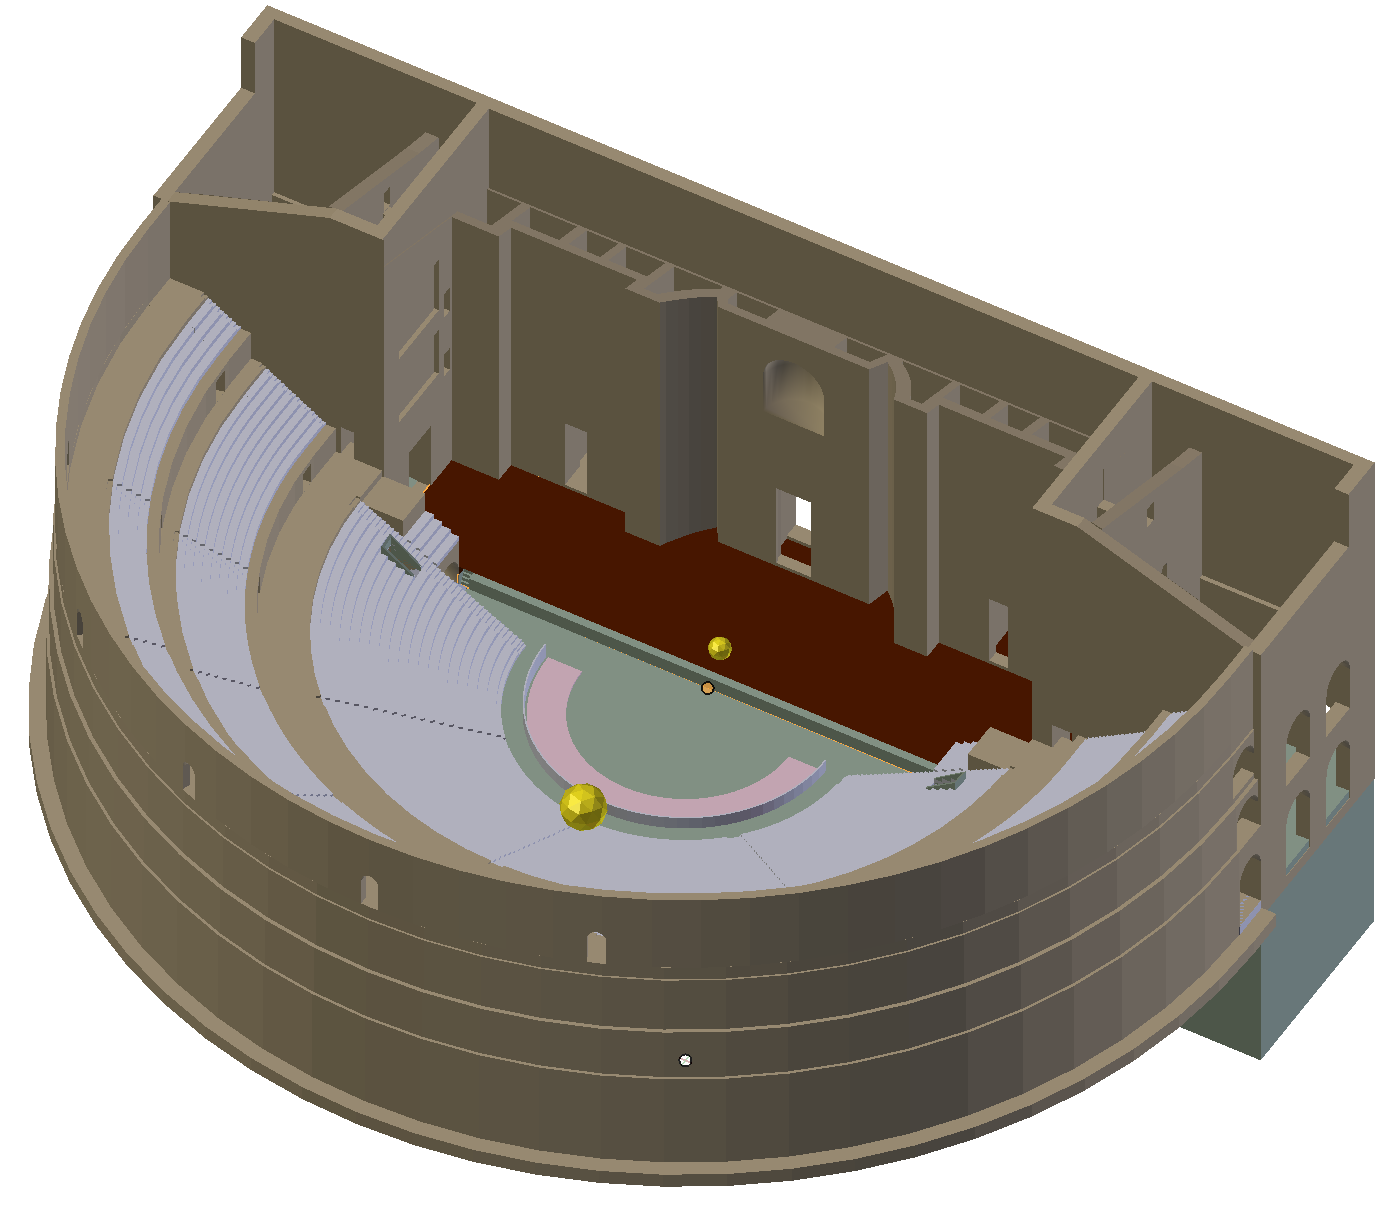
\includegraphics[width=\linewidth]{images/theatreMat}
	\caption{Représentation des matériaux sur le théâtre d'Orange : Calcaire (beige), Marbre (vert), Bois (orange), Audience sur gradins (gris), Audience sur siège en bois (rose) ainsi que la source (rouge) et le récepteur (jaune) dans la configuration initiale.}
	\label{theatreMat}
\end{figureth}

On peut voir sur la figure \ref{theatreMat} la répartition des différents matériaux sur le bâtiment. Nous plaçons une source sonore centrée sur la largeur de la scène à 160cm au dessus de celle-ci (environ la hauteur d'une bouche humaine) soit à une altitude de 42,8m par rapport au niveau de la mer (voir section \ref{sect_methodo}) et à 2m du bord. Nous choisissons cette position comme position de source initiale. Le récepteur initial est situé dans le même axe, c'est-à-dire au centre des gradins et à la même altitude. Sa distance par rapport au centre de l'orchestre est de 16,5m, ce qui correspond aux gradins 3 à 8 environ. Son rayon de mesure sera de 2m. 

Nous testons le calcul complet avec respectivement un et deux millions de rayons. Nous constatons que les résultats sont quasiment identiques à partir de 500Hz mais que les temps de réverbération sont un peu plus grands pour les basses fréquences à deux millions de rayons (moins de 10\% d'écart). Cela s'explique par le fait que l'atmosphère ainsi que les matériaux atténuent très peu ces fréquences. Cependant, ce faible écart de résultats reste acceptable compte tenu de la diminution du temps de calcul. Afin de calculer les configurations correspondantes, il faut respectivement 17min pour deux millions de rayons et 8min pour un million. Nous testons aussi le calcul avec 500~000 rayons, pour lequel temps de calcul est de 3min et retrouvons des résultats identiques à la configuration à deux millions de rayons seulement au delà de 4kHz. Pour les plus basses fréquences l'écart va jusqu'à 17\%. Dans la suite, nous choisissons donc de travailler avec un million de rayons.



\section{Analyse de la réponse impulsionnelle} \label{sect_analyse_rir}

%L'analyse de l'acoustique d'une salle peut se faire à l'aide de différents facteurs perceptifs tel que le \gls{RT60} que nous avons décrit précédemment. 
%La \gls{rir} de la configuration décrite précédemment pour un \gls{RT60} est présentée figure \ref{rirTheatre}.

\begin{figureth}
	\begin{subfigureth}{\linewidth}
		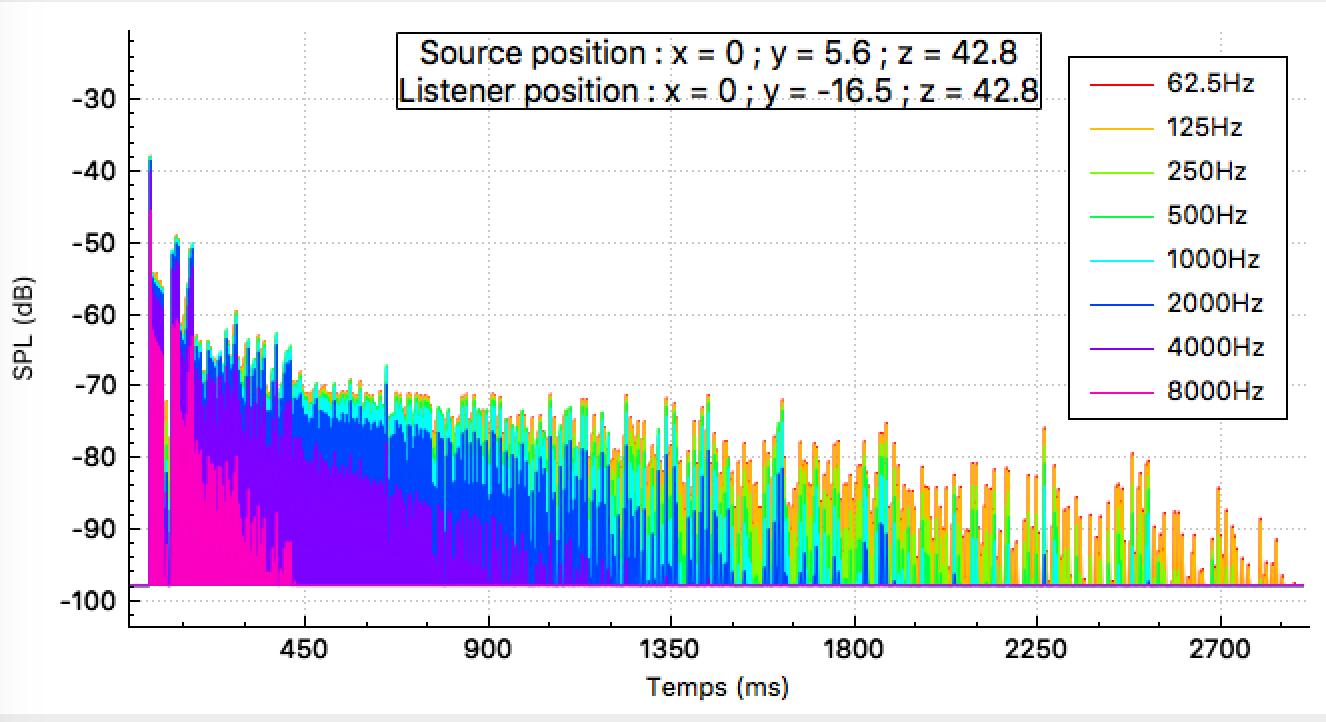
\includegraphics[width=\linewidth]{images/rirTheatreAvecDecor}
			\caption{Réponse impulsionnelle jusqu'à -60dB.}
		\label{rirTheatre60}
	\end{subfigureth}
		\begin{subfigureth}{\linewidth}
		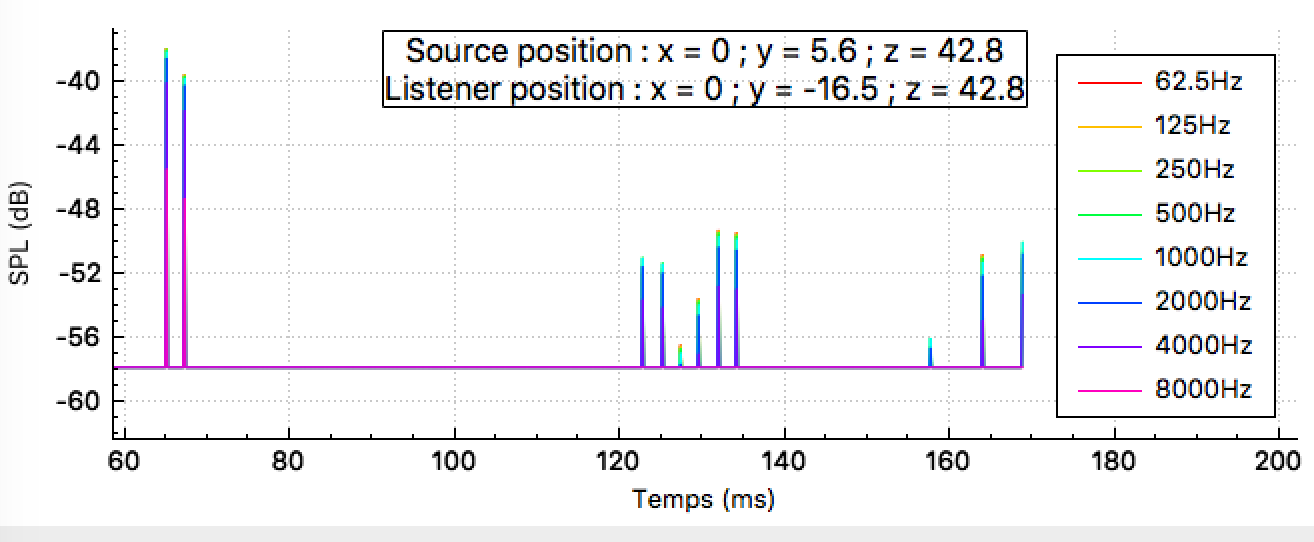
\includegraphics[width=\linewidth]{images/rirTheatre20}
		\caption{Réponse impulsionnelle jusqu'à -20dB.}
		\label{rirTheatre20}
	\end{subfigureth}
	\caption{\gls{rir} du théâtre d'Orange dans sa configuration initiale pour 1 million de rayons.}
	\label{rirTheatre}
\end{figureth}

La figure \ref{rirTheatre} et le tableau \ref{tab_fact_init} illustrent les caractéristiques de la réponse impulsionnelle de la configuration initiale. On constate une zone de premières réflexions jusqu'à 400ms puis une chute d'énergie pour le champ diffus qui s'étale au delà des 3 secondes pour atteindre le \gls{RT60}. Nous limitons la réponse impulsionnelle à -20dB afin d'analyser d'où proviennent les pics d'énergies les plus forts (voir fig. \ref{rirTheatre20}). Pour cela, nous nous appuyons sur les travaux de Haas et Meyer \cite[p.49]{haas} qui expliquent à quel moment une réflexion devient un écho :
\begin{itemize}
\item si l'intervalle entre le son direct et le son réfléchi est inférieur à 5ms, l'auditeur entend un son unique dont l'intensité est la somme des deux signaux. La direction perçue est la bissectrice de l'angle formé par les deux sources (réelle et virtuelle) ;
\item si le temps entre les deux signaux est compris ente 5 et 35ms, l'intensité est encore la somme des intensités mais la direction est celle du premier signal ;
\item si le temps entre les deux signaux est compris entre 35 et 50ms, les deux signaux sont distingués dans le temps mais la direction semble être celle du premier son ;
\item au delà de 50ms, les deux signaux sont complètement distingués dans le temps et l'espace.
\end{itemize}
Sur la figure \ref{rirTheatre20} on constate la présence d'un pic de signal 5ms après le son direct ce qui entre dans le premier cas décrit précédemment. Après analyse, nous constatons que celui-ci provient de la réflexion sur l'orchestre. Celui-ci va donc doubler l'intensité sonore émise depuis l'avant scène. Ce phénomène semble avoir été bien maitrisé par les architectes de l'antiquité comme le montre l'exemple du théâtre de Dyonisos en Grèce (voir fig. \ref{dyonisos}). Celui-ci possède un losange dessiné sur son orchestre qui semble représenter l'espace qui ne doit pas est recouvert afin que le son puisse s'y réfléchir \cite[p.118-120]{canac}. Si on limite la réponse impulsionnelle à -30dB (voir fig. \ref{rirTheatre30}), nous constatons qu'il y a ensuite beaucoup de signal dispersé sur environ 30ms qui correspond aux rayons réfléchis sur le dossier des gradins et qui reviennent converger sur le récepteur (voir fig \ref{SI30dB}). Une partie d'entre eux se sont également réfléchis sur l'orchestre ajoutant encore à l'impact de cette surface dallée. D'après les critères de Haas évoqués précédemment, ces signaux sont parfaitement confondus avec le son direct. Il y a ensuite un trou de 20ms avant les prochains pics. Ceux-ci étant retardés de plus de 50ms par rapport au son direct, ils pourront être perçus comme un écho. Ces derniers proviennent des réflexions sur les marches d'escalier de la porte royale. Il est bon de rappeler que nous utilisons une source omnidirectionnelle et qui, à la différence de la voix humaine envoie autant d'énergie vers le mur que vers les gradins. Par ailleurs, nous sommes dans l'approximation hautes fréquences où l'on néglige certains effets de diffraction. On peut donc s'attendre à avoir un signal un peu différent dans la réalité même si notre étude permet de se faire une bonne idée du comportement acoustique du bâtiment. À 160ms les quelques pics présents sont dûs aux rayons réfléchis sur les gradins qui, bien que fortement atténués par le matériau, arrivent en phase et jouent donc un rôle non négligeable dans la réverbération (voir fig. \ref{SI30dB}). Il y a ensuite deux grands pics à -10dB issus de multiples réflexions. Le premier est dû aux réflexions successives sur le \gls{balteus}, le fond du \gls{pulpitum} et l'orchestre. Le deuxième provient de réflexions au niveau de la porte royale et de l'orchestre. L'agencement de ces deux parties (le \gls{balteus} et la porte royale) étant très hypothétiques, il faudra considérer la présence de ces deux pics comme peu fiable. Pour finir, on distingue quatre grands pics provoqués par les réflexions sur le plafond de la scène ainsi que des combinaisons de réflexions avec la scène et les basiliques. Les deux premiers vont difficilement être distingués des pics précédents car leur écart est inférieur à 35ms mais les deux derniers seront entendus comme un écho.
\begin{figureth}
	\begin{subfigureth}{0.48\textwidth}
		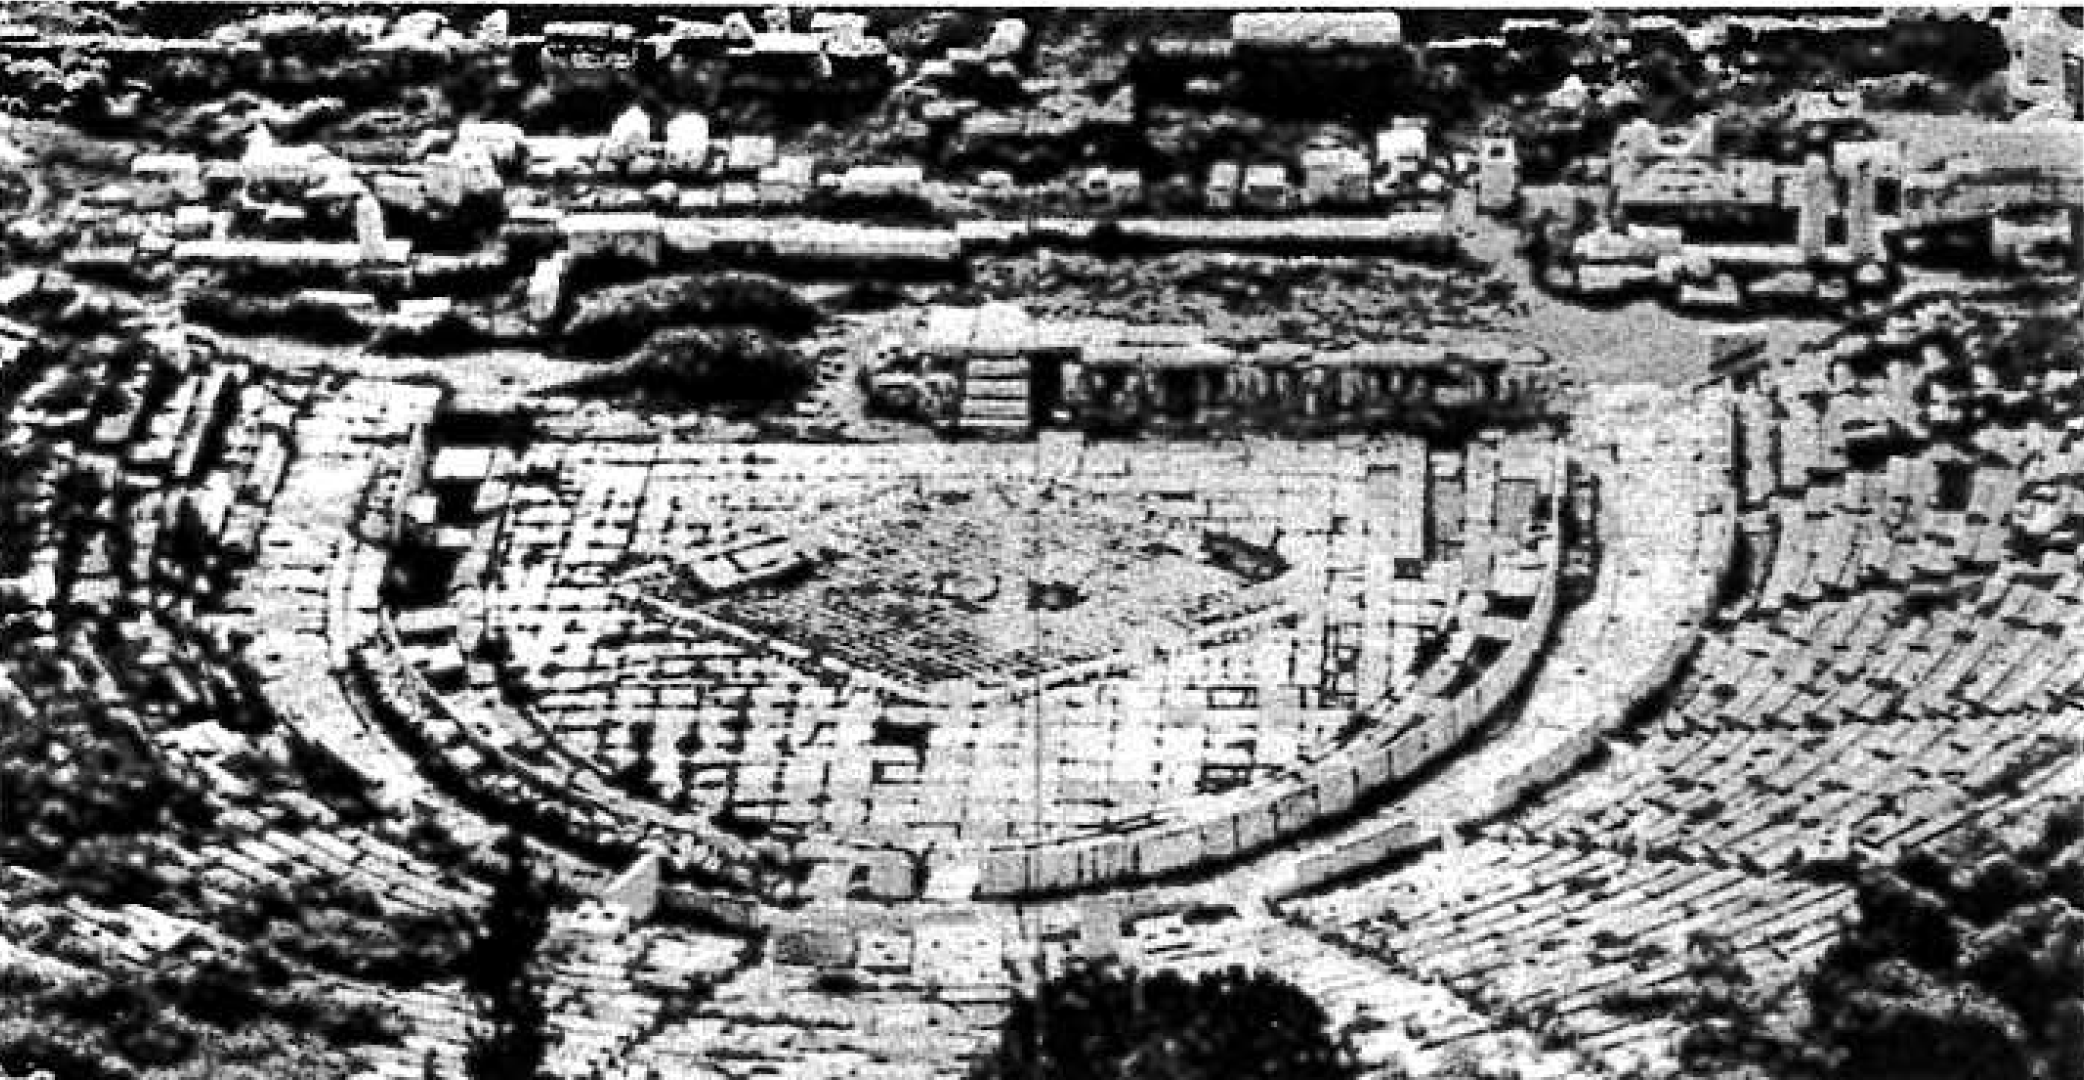
\includegraphics[width=\linewidth]{images/dyonisos1}
		\caption[Mosaïque en losange dans l'orchestre du théâtre de Dyonisos à Athènes.]{Mosaïque en losange dans l'orchestre du théâtre de Dyonisos à Athènes \footnotemark.}
		\label{dyonisos1}
		\hfill
		\quad
	\end{subfigureth}
	\quad
	\begin{subfigureth}{0.48\textwidth}
		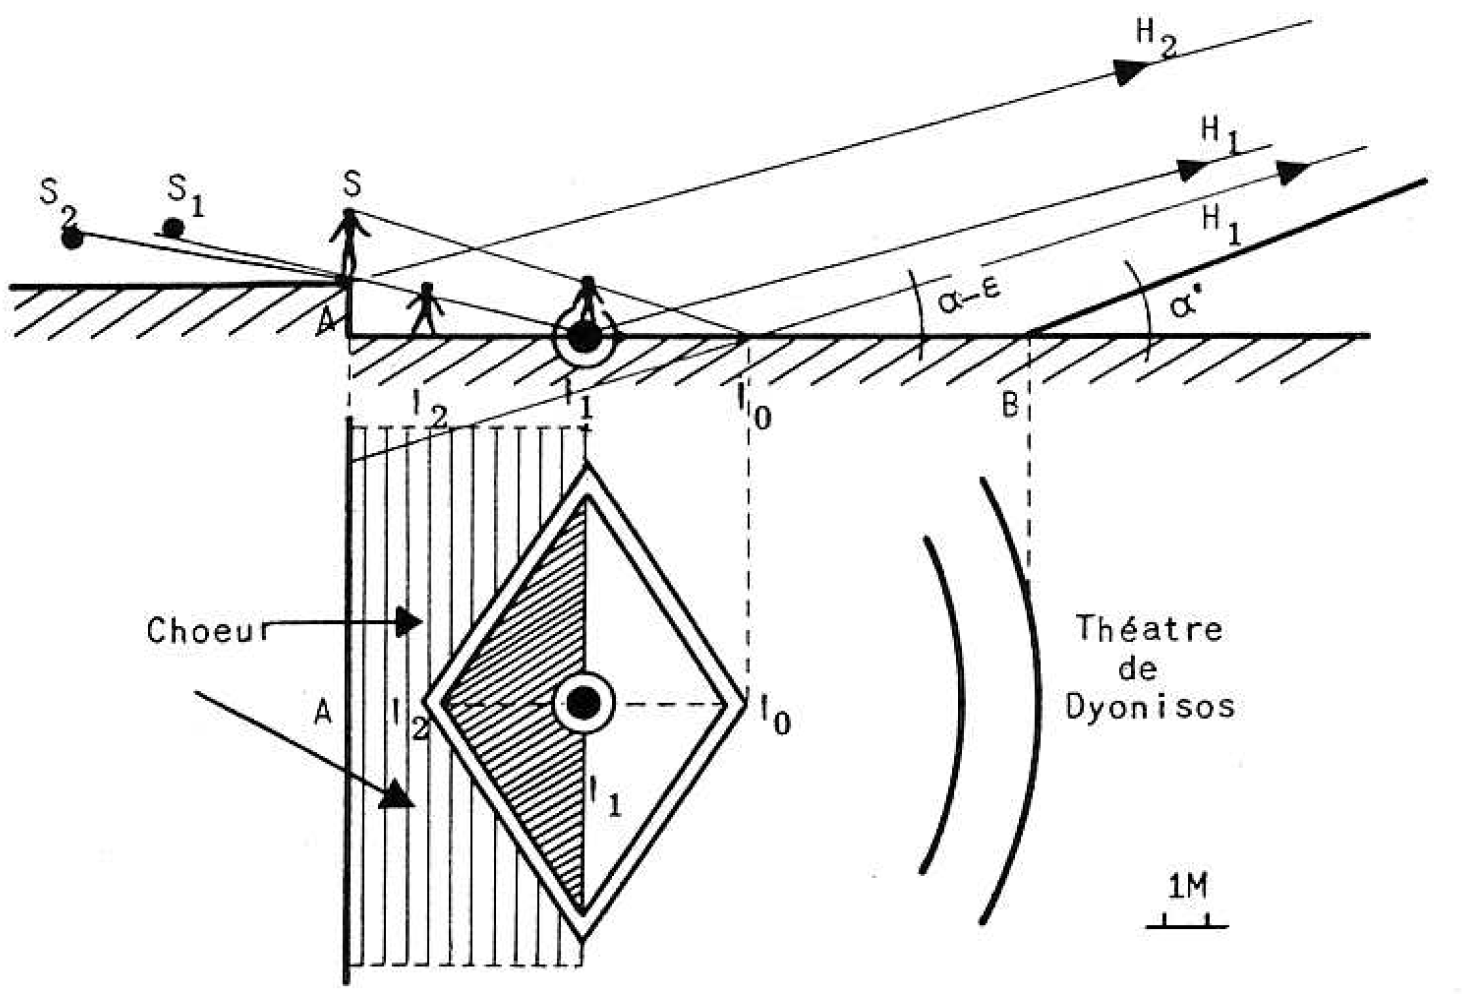
\includegraphics[width=\linewidth]{images/dyonisos2}
		\caption[Rôle supposé du losange dans l'orchestre du théâtre de Dyonisos. Emplacement du choeur.]{Rôle supposé du losange dans l'orchestre du théâtre de Dyonisos. Emplacement du choeur \footnotemark.}
		\label{dyonisos2}
		\quad
	\end{subfigureth} 
\caption{Analyse de l'orchestre du théâtre de Dyonisos à Athènes.}	
\label{dyonisos}
\end{figureth}	
\addtocounter{footnote}{-1}
\citefnt[Fig. V-7 bis - p.119]{canac}
\addtocounter{footnote}{1}
\citefnt[Fig. V-7 - p.118]{canac}
% 
\begin{figureth}
	\begin{subfigureth}{\linewidth}
		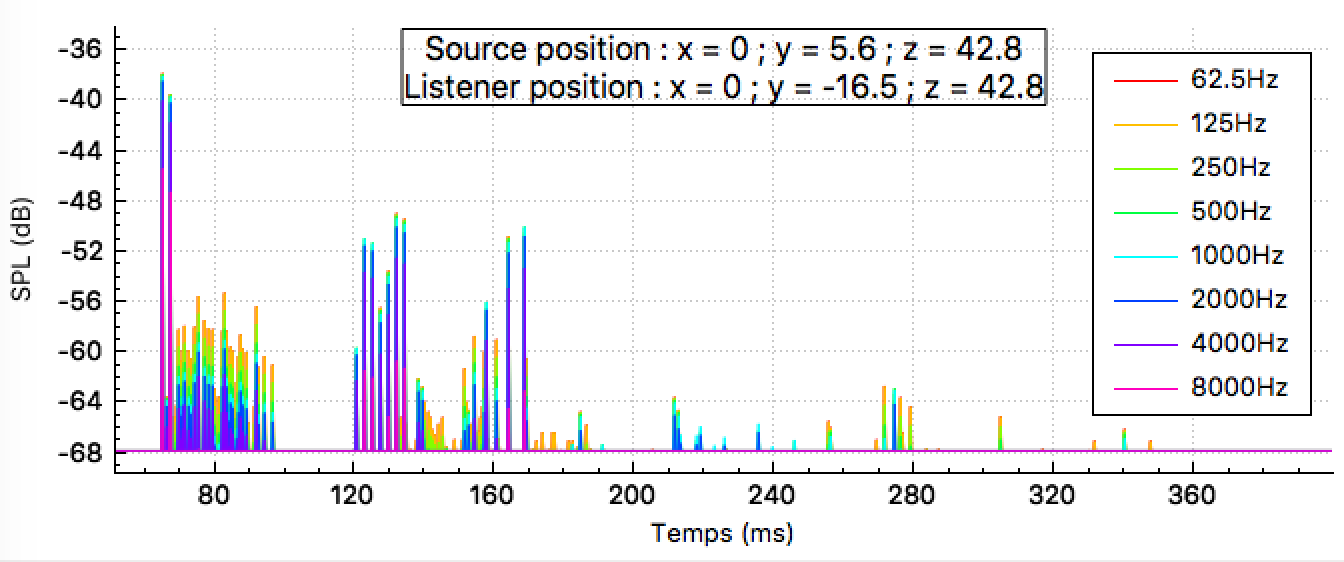
\includegraphics[width=0.85\linewidth]{images/rirTheatre30}
		\caption{Réponse impulsionnelle jusqu'à -30dB.}
		\label{rirTheatre30}
	\end{subfigureth}
	\begin{subfigureth}{0.36\textwidth}
		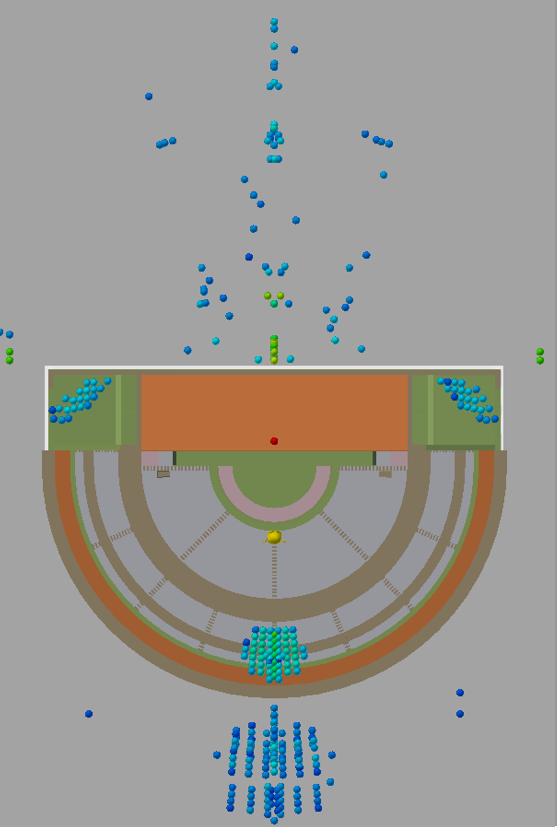
\includegraphics[width=\linewidth]{images/SI30dBbis}
		\caption{Source-images spatialisées jusqu'à -30dB.}
		\label{SI30dBbis}
	\end{subfigureth}
	\begin{subfigureth}{0.61\textwidth}
		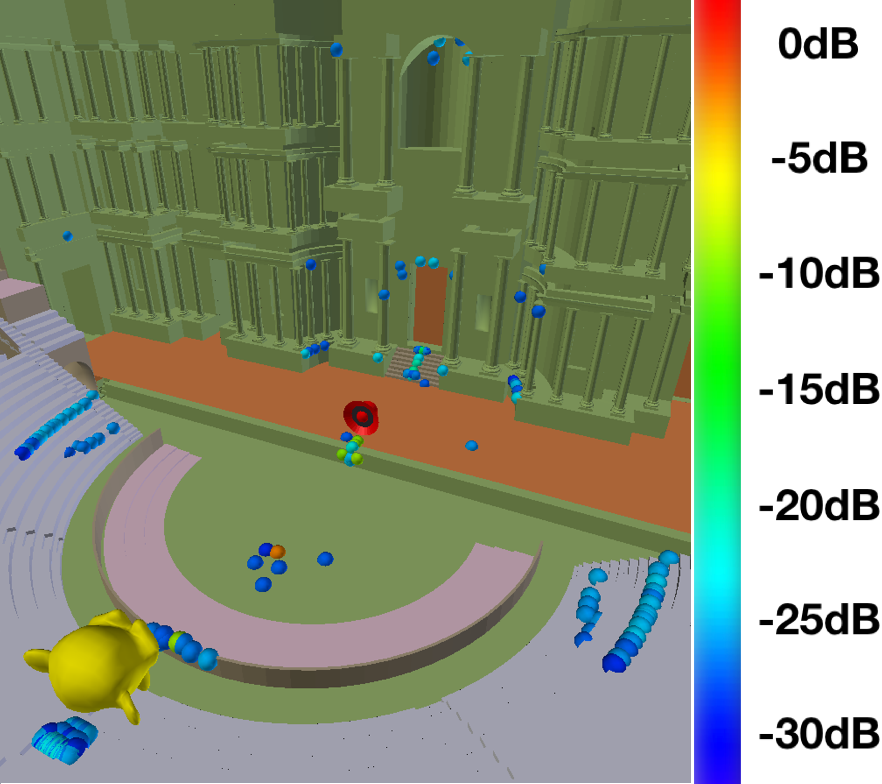
\includegraphics[width=\linewidth]{images/SI30dB}
		\caption{Source-images projetées sur les parois du théâtre jusqu'à -30dB.}
		\label{SI30dB}
	\end{subfigureth}
\caption{La \gls{rir} et ses sources-images dans le théâtre d'Orange dans sa configuration initiale pour 1 million de rayons jusqu'à -30dB.}	
\label{SITheatre30}
\end{figureth}
%


\begin{figureth}
	\begin{subfigureth}{0.8\textwidth}
		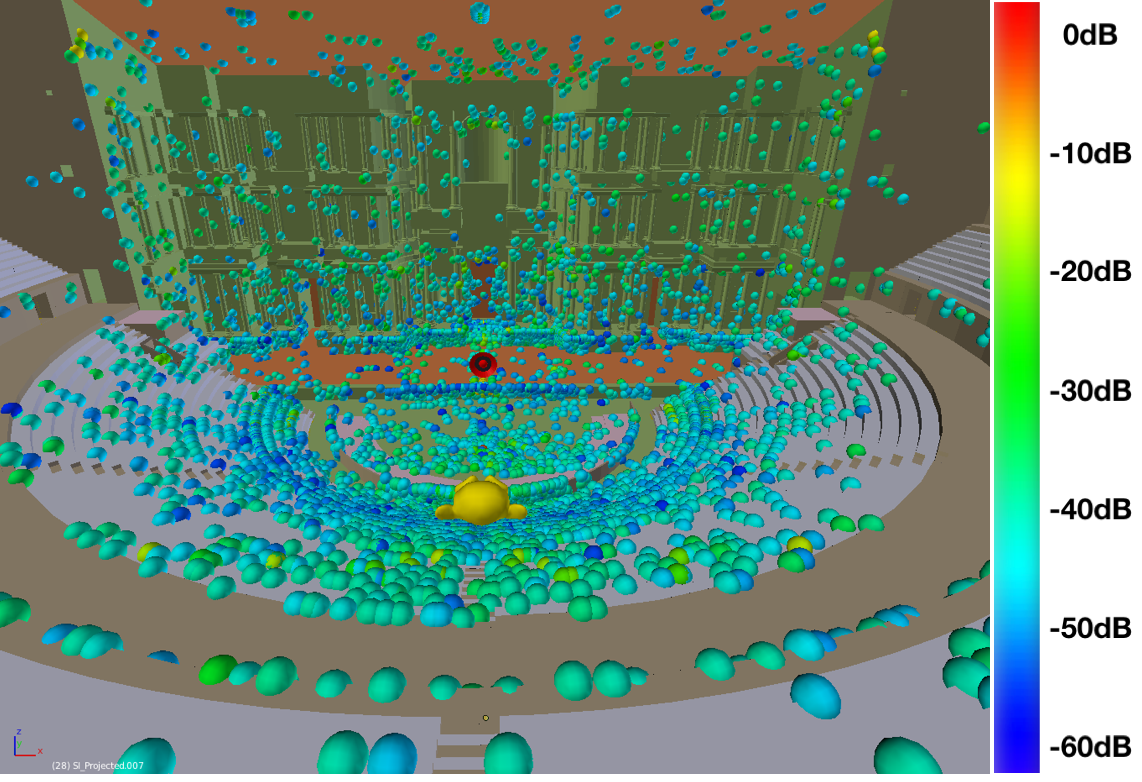
\includegraphics[width=\linewidth]{images/SI60dB}
		\caption{Source-images projetées sur les parois du théâtre jusqu'à -60dB vues des gradins.}
		\label{SI60dB}
		\hfill
		\quad
	\end{subfigureth}
	\begin{subfigureth}{0.8\textwidth}
		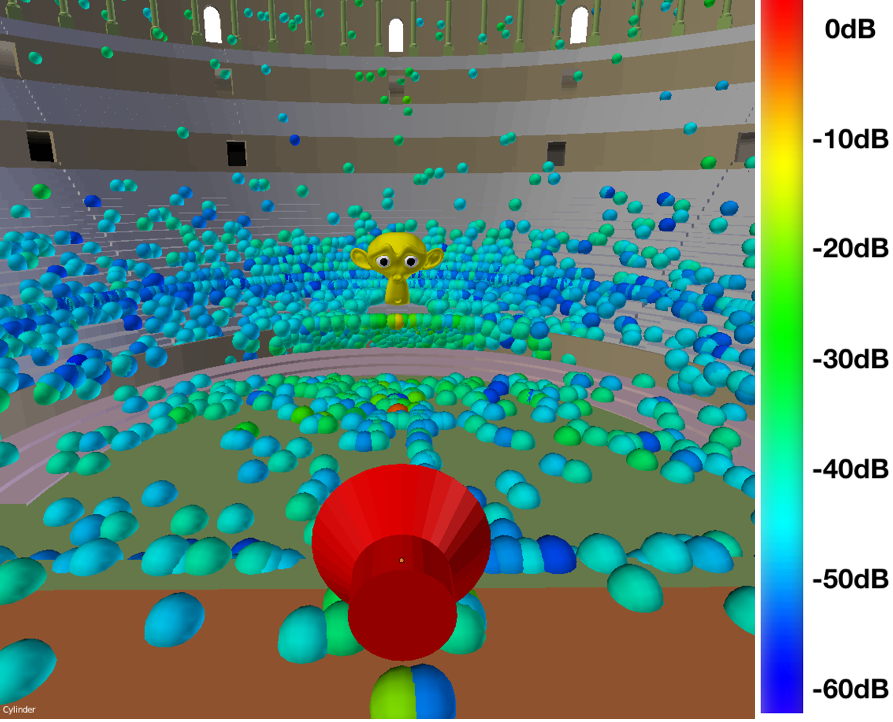
\includegraphics[width=\linewidth]{images/SI60dBbis}
		\caption{Source-images projetées sur les parois du théâtre jusqu'à -60dB vues de la scène.}
		\label{SI60dBbis}
		\quad
	\end{subfigureth} 
\caption{Source-images dans le théâtre d'Orange dans sa configuration initiale pour 1 million de rayons.}	
\label{SITheatre60}
\end{figureth}
%
En ce qui concerne la position des sources-images, on constate clairement que pour une mesure à -60dB, il y a des sources-images tout autour du récepteur avec de fortes concentrations sur les premiers gradins, sur l'orchestre, sur la scène et sur le bas du mur (voir fig. \ref{SI60dB}). C'est finalement à proximité du plan source-récepteur que se concentre la majeure partie des sources-images. Cependant, on constate la présence de sources-images au niveau du plafond, de la niche centrale et des différentes \glspl{precinction} ce qui implique que le son qui monte peut aussi redescendre vers les gradins du bas (voir fig. \ref{SI60dBbis}). En observant les sources-images dont le niveau est supérieur à -30dB par rapport au son direct (voir fig. \ref{SITheatre30}), on peut confirmer la provenance des pics d'énergie de la figure \ref{rirTheatre30} décrite précédemment. 



La tableau \ref{tab_fact_init} présente les facteurs perceptifs de cette configuration initiale. Ces données confirment un temps de réverbération de l'ordre de 4s. Il est intéressant de constater que ce temps est supérieur du temps de réverbération optimal pour la parole décrit par J. Jouhaneau \cite[p.209]{jouhaneau} et qui se trouve être légèrement inférieur à 2s. Ce dernier est obtenu à partir des courbes de pourcentage d'intelligibilité et de niveau sonore qui se croisent en ce point optimal. En effet, la réverbération d'une salle permet d'amplifier le niveau sonore de la voix, donc d'être mieux entendu mais, lorsque le signal se diffuse plus longtemps, il devient plus difficile de dissocier et comprendre les mots. Le temps optimal est déterminé empiriquement et peut être discutable puisque J. Jouhaneau décrit lui-même les limites de cette analyse dépendant du volume et du signal émis \cite[p.218]{jouhaneau}. Ce manque de compréhensibilité est corroboré par l'analyse des autres facteurs. Tout d'abord, on constate que la définition \gls{D50} et la clarté \gls{C80} augmentent avec la fréquence. Nous savons que les hommes, lorsqu'ils utilisent une voix de poitrine, émettent des fréquences de 80 à 400Hz environ tandis que les femmes, en voix de têtes, émettent des fréquences de 300 à 1500Hz \cite[Mécanismes vocaux]{voix}. Cependant, seuls les hommes étaient acteurs de théâtre à l'époque impériale. On en conclut que la compréhensibilité de leur voix n'était pas excellente mais plutôt moyenne. Le théâtre semble donc un peu mieux adapté à la musique qu'au texte puisqu'il est dit que pour une écoute musicale optimale, la clarté doit se situer entre -3dB et +3dB \cite[p.59]{acoustique}. Le temps central \gls{Ts} étant supérieur à 50ms et l'\gls{EDT} étant supérieur à 1s, on comprend d'autant plus que le signal va s'étaler et que les syllabes seront peu distinctes. En ce qui concerne le niveau sonore, on constate que le théâtre présente un gain compris entre 3 et 6dB selon la fréquence. Cela signifie que le bâtiment a un effet bénéfique pour la transmission du son puisqu'il double le niveau sonore des plus hautes fréquences et quadruple celui des basses fréquences. On retrouve bien l'analyse faite précédemment sur l'orchestre qui double le niveau sonore de la source. Le \gls{LF80} nous indique, quant à lui, une sensation d'éloignement par rapport à la source, ce qui n'est pas étonnant au vu des dimensions du théâtre.
%
\begin{tableth} 
 \begin{tabular}{| *{9}{c|}} 
 \hline 
 Facteur & 62,5Hz & 125Hz & 250Hz & 500Hz & 1kHz & 2kHz & 4kHz & 8kHz \\ 
 \hline 
 \hline 
\gls{EDT} (ms)& 2061& 2039& 1890& 1854& 1750& 1452& 1206& 416 \\ 
 \hline 
\gls{T30} (ms)& 4159& 4106& 3819& 3591& 3210& 2455& 1474& 685 \\ 
 \hline 
\gls{RT60} (ms)& 3791& 3755& 3554& 3408& 3169& 2561& 1549& 661 \\ 
 \hline 
\gls{spl} (dB)& -31& -31& -31& -32& -32& -33& -35& -42 \\ 
 \hline 
\gls{G} (dB)& 7& 7& 6.7& 6.5& 6.2& 5.8& 5& 3.6 \\ 
 \hline 
\gls{C80} (dB)& 0.8& 0.84& 1.07& 1.12& 1.38& 2.16& 4.2& 10.2 \\ 
 \hline 
\gls{D50} (\%)& 46.26& 46.46& 47.32& 47.19& 48.47& 52.44& 62.67& 84.08 \\ 
 \hline 
\gls{Ts} (ms)& 133& 132& 121& 117& 110& 91& 58& 19 \\ 
 \hline 
\gls{LF80} (dB)& 0.003& 0.003& 0.003& 0.002& 0.002& 0.002& 0.001& 0.001 \\ 
 \hline 
\end{tabular}
 \caption{Facteurs perceptifs pour une source en [0 ; 5.6 ; 42.8] et un auditeur en [0 ; -16.5 ; 42.8] et 1000000 rayons dans la configuration initiale.} 
 \label{tab_fact_init} 
 \end{tableth}

Pour résumer, dans une configuration d'utilisation que l'on considère comme standard, le théâtre amplifie le volume sonore mais la présence de quelques échos dégrade la transmission du texte. Si l'on devait comparer le théâtre d'Orange à une salle de spectacle moderne par la seule lecture de ses facteurs perceptifs, il se rapprocherait plutôt d'un opéra que d'un théâtre. C'est  à partir de cette analyse initiale que nous allons pouvoir comparer différentes configurations du bâtiment et en déterminer l'impact sur l'acoustique.


		
\chapter{Test de configurations}
	\citationChap{
Don't stop me now \\
I'm having such a good time
		}{Queen}
	\minitoc
	\newpage

\section{Décor du front de scène}

Comme nous l'avons évoqué en introduction de ce chapitre, l'acoustique du théâtre d'Orange a déjà été étudiée par F. Canac dans les années 1960. Le problème de cette étude est qu'elle se base sur le théâtre tel qu'il existe aujourd'hui, c'est-à-dire dépouillé de l'ornementation du front de scène. Pour pouvoir comparer nos résultats à cette étude, nous ôtons la décoration du mur de scène ainsi que la \gls{porticus isc} et le toit au dessus de la scène. Nous pouvons alors mesurer la réponse impulsionnelle du théâtre dans un état proche de celui d'aujourd'hui. Le tableau \ref{tab_fact_sansdec} présente les facteurs perceptifs de cette configuration sans décor. En les comparant au tableau \ref{tab_fact_init}, on constate que retirer le décor améliore la clarté \gls{C80} puisque cette configuration gagne 3 à 4dB et que la définition \gls{D50} passe au dessus de 60\% quelle que soit la fréquence. Les facteurs \gls{EDT} et \gls{Ts} nous permettent de comprendre que les échos les plus forts parviennent plus rapidement à l'auditeur. Le décor a donc un effet de diffusion du son, ce qui est favorable à l'écoute musicale mais dégrade la transmission de la parole. Il est intéressant de constater que c'est exactement le contraire de ce qu'expliquait Formigé au début du $XX^e$ siècle : " le \textit{frons scaenae} renvoyait le son sans échos, après les avoir brisés grâce à la multiplicité des plans et des ornements" \cite[p.43]{formige}. Notons pour finir que les facteurs qui ne sont pas présentés dans tableau \ref{tab_fact_sansdec}, tel que le \gls{LF80} par exemple, restent très similaires à la configuration initiale.%


\begin{figureth}
	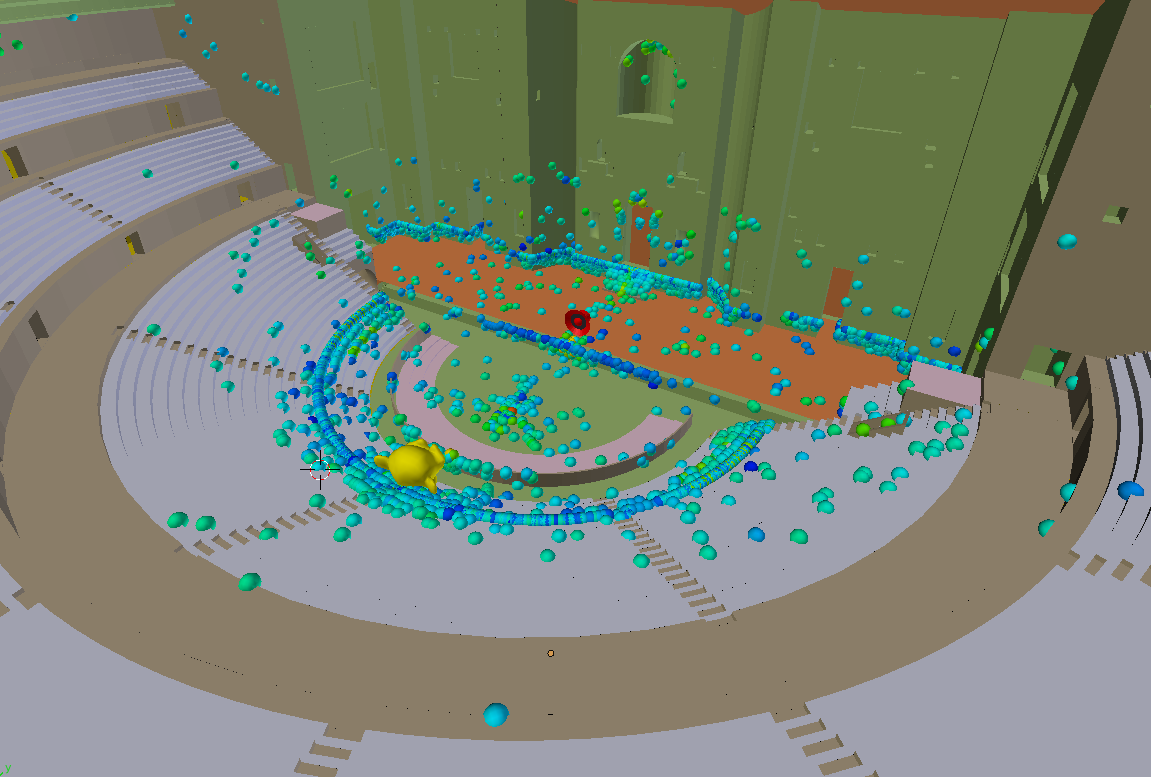
\includegraphics[width=\linewidth]{images/SIsansDec}
	\caption{Source-images projetées sur les parois du théâtre jusqu'à -60dB sans la décoration du front de scène.}
	\label{SIsansDec}
\end{figureth}

\begin{tableth} 
 \begin{tabular}{| *{9}{c|}} 
 \hline 
 Facteur & 62,5Hz & 125Hz & 250Hz & 500Hz & 1kHz & 2kHz & 4kHz & 8kHz \\ 
 \hline 
 \hline 
\gls{EDT} (ms)& 1436& 1387& 1211& 884& 709& 645& 594& 361 \\ 
 \hline 
\gls{T30} (ms)& 3886& 3827& 3049& 2745& 2477& 1969& 1315& 592 \\ 
 \hline 
\gls{G} (dB)& 5.8& 5.8& 5.4& 5& 4.8& 4.6& 4.1& 3.4 \\ 
 \hline 
\gls{C80} (dB)& 4.01& 4.04& 4.83& 5.41& 5.89& 6.68& 8.51& 13.37 \\ 
 \hline 
\gls{D50} (\%)& 61.01& 61.17& 63.81& 65.42& 67.04& 69.84& 76.22& 88.34 \\ 
 \hline 
\gls{Ts} (ms)& 84& 83& 68& 60& 53& 44& 28& 12 \\ 
 \hline 
\end{tabular} 
 \caption{Facteurs perceptifs pour une source en [0 ; 5.6 ; 42.8] et un auditeur en [0 ; -16.5 ; 43.9] et 1~000~000 de rayons sans décoration du front de scène.} 
 \label{tab_fact_sansdec} 
 \end{tableth}


\section{Position des spectateurs} \label{sect_positionSpectateur}
Le test suivant consiste à comprendre l'impact de la position dans les gradins. Nous savons que le placement dans la \gls{cavea} se faisait selon le rang social des spectateurs. Nous comprenons facilement que visuellement, les spectateurs les plus proches étaient ceux qui voyaient le mieux les acteurs, même si ceux situés légèrement en recul avaient une meilleure vue d'ensemble. Ainsi, nous avions les sénateurs sur des sièges mobiles dans l'orchestre, les chevaliers sur les premiers gradins, puis la plèbe et pour finir les esclaves. Les tribunes étaient également occupées par des personnages importants.

Nous testons donc 12 nouvelles positions d'auditeurs afin de comparer le signal perçu avec la \gls{rir} de référence (voir fig. \ref{position_rece}). Nous positionnons des séries d'auditeurs sur des axes à 0°, 55° et à 90° par rapport à la perpendiculaire au mur de scène. Sur chacun de ces axes, on positionne des récepteurs sur les derniers gradins de chaque \gls{maenianum} et pour les axes n'étant pas au niveau de l'\gls{aditus}, on ajoute également des récepteurs au niveau des premiers gradins et de ceux de l'orchestre. On notera que les récepteurs 1, 5, 6 et 10 sont situés à l'emplacement de personnalités importantes. Nous affichons les données sur la plage de fréquence de 500 à 1000Hz car elle semble assez centrale. Les résultats relatifs (c'est-à-dire en comparant les auditeurs les uns par rapport aux autres) sont assez similaires pour les autres fréquences. Notons que le calcul pour l'ensemble des récepteurs s'effectue en une dizaine de minutes.
\begin{figureth}
	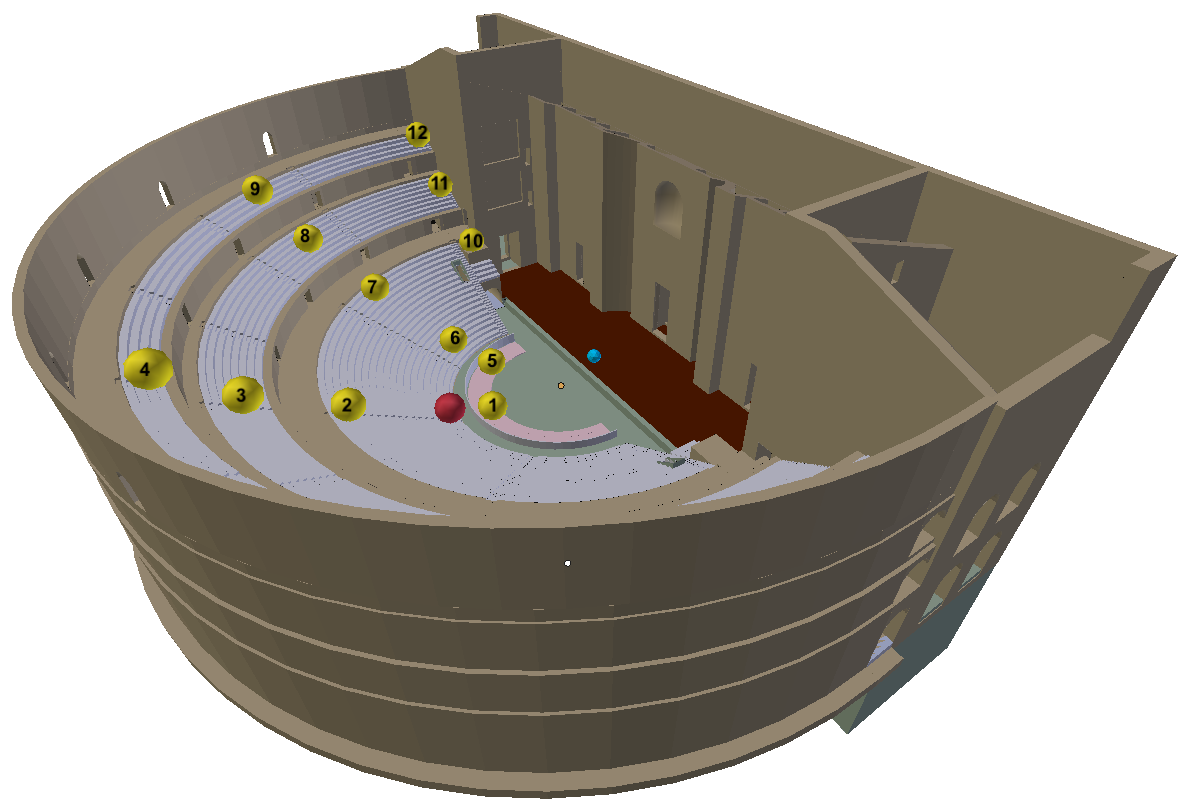
\includegraphics[width=\linewidth]{images/position_rece}
	\caption{Douze positions d'auditeurs (rose) à comparer à la position initiale (jaune).}
	\label{position_rece}
\end{figureth}
%
\begin{tableth} 
\footnotesize
 \begin{tabular}{| *{9}{c|}} 
 \hline 
 Récepteur & [x ; y ; z] (m)  & \gls{EDT} (ms) & \gls{T30} (ms) & \gls{spl} (dB) & \gls{C80} (dB) & \gls{D50} (\%) & \gls{Ts} (ms) \\ %& \gls{LF80} (dB) \\ 
 \hline 
 \hline 
1  & [0 ; -10.67 ; 41.44] &1668  &3465   &-28  &1.63  &53.62  &107 \\%listener12
 \hline 
 Réf    &[0 ; -16.5 ; 43.9] &1854  &3591   &-32  &1.12  &47.19  &117 \\%listener0-REF
 \hline 
 2  & [0 ; -28.23 ; 50.02] &2572  &4235   &-34  &0.15  &37.96  &154 \\ %listener11
 \hline 
 3  &  [0 ; -37.86 ; 55.92] &2462  &4719   &-36  &-0.85  &32.66  &156 \\ %listener10
 \hline 
 4  &  [0 ; -44.36 ; 62.06] &2827  &4500   &-36  &-1.67  &30.64  &176 \\%listener9
 \hline 
 \hline
 5  &   [-8.74 ; -6.12 ; 41.44] &1851  &3470   &-27  &2.6  &56.79  &102 \\%listener5
 \hline 
 6  &  [-13.51 ; -9.46 ; 43.86] &1892  &3994   &-31  &2.77  &56.06  &108 \\%listener4
  \hline 
  7 &   [-23.12 ; -16.19 ; 50.02] &2439  &4497   &-33  &0.64  &42.03  &153 \\ %listener6
 \hline 
 8  &  [-31.02 ; -21.72 ; 55.92] &2693  &4514   &-36  &0.02  &43.55  &170 \\ %listener7
 \hline 
 9  & [-36.34 ; -25.44 ; 62.06] &3225  &4416   &-37  &-1.16  &32.49  &205 \\ %listener8
 \hline 
 \hline
 10  &  [-28.23 ; 1.66 ; 50.02] &3255  &4466   &-32  &-2.56  &29.46  &203 \\ %listener3
 \hline 
11   & [-37.87 ; 1.66 ; 55.92] &3840  &4104   &-36  &-2.16  &35  &258 \\%listener2
 \hline 
12   & [-44.36 ; 1.66 ; 62.06] &4410  &4664   &-36  &-3.32  &28.64  &299\\ %listener1
 \hline 
\end{tabular} 
 \caption{Facteurs perceptifs pour différents récepteurs sur la bande de fréquence de 500Hz pour 1~000~000 de rayons.} 
 \label{tab_fac_rec} 
 \end{tableth}
 
 
On constate d'après le tableau \ref{tab_fac_rec} plusieurs choses. Tout d'abord, le niveau acoustique \gls{spl} diminue de 4dB entre les gradins mobiles de l'orchestre réservés aux sénateurs et les premiers gradins accessibles aux classes moins élevés tels que les chevaliers. Le son est donc entendu environ deux fois moins fort. La perte est de 10dB au sommet de la \gls{cavea} ce qui implique que les classes les plus modestes entendaient le son de la scène dix fois moins fort que les sénateurs de l'orchestre. En ce qui concerne la compréhensibilité, on distinguera les récepteurs situés au dessus de l'\gls{aditus} des autres. Ainsi on constate d'après les facteurs de clarté (\gls{C80}) et de définition (\gls{D50}) que pour les récepteurs 10 à 12 la compréhensibilité est nettement dégradée. On comprend grâce à la figure \ref{listener11} que cela est dû principalement aux deux \glspl{basilique}. Celle située à l'est génère un fort écho éloigné du son direct de la largeur de la scène (alors que pour les récepteurs dans l'axe, l'écho généré par le mur de scène n'est séparé que par la profondeur de la scène). On a aussi une forte concentration de sources-images au niveau de la \gls{precinction} à l'est du théâtre. La basilique occidentale va quant à elle stocker le son plus longtemps comme une sorte d'entonnoir puisque l'auditeur est dans son angle. Nous pouvons également noter que la première réflexion qui se fait sur l'orchestre lorsqu'on est dans la \gls{cavea} se fait sur la scène lorsqu'on est au dessus des \glspl{aditus}. L'effet miroir est donc légèrement estompé. Au niveau de la tribune, donc du récepteur 10 (voir fig. \ref{listener10}), l'effet est différent puisque le son provient principalement de la partie occidentale du front de scène, le plafond et l'arrière de la tribune. Cela doit être particulièrement bien adapté pour l'écoute musicale mais est finalement une des plus mauvaise place pour l'écoute de la parole.
On analyse par ailleurs que, quel que soit l'axe, lorsqu'on s'éloigne de la scène, le temps de réverbération augmente globalement. Cela est dû au fait que les divers réflexions entre le mur de scène et l'arrière de l'auditeur sont plus longues lorsqu'on s'éloigne du mur. Les autres facteurs permettent de comprendre que la compréhensibilité se dégrade aussi avec l'éloignement. 
\begin{figureth}
	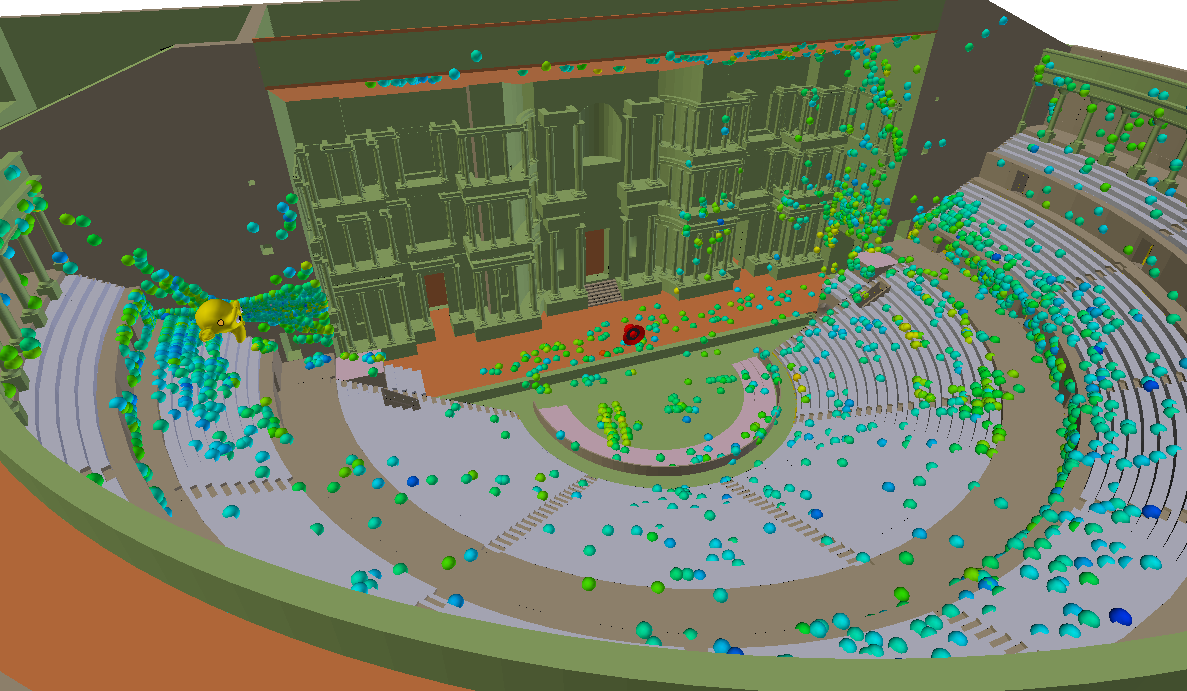
\includegraphics[width=\linewidth]{images/Listener11}
	\caption{Projection des sources-images pour un auditeur situé sur le deuxième \gls{maenianum} au dessus de l'\gls{aditus} occidental pour 1~000~000 de rayons.}
	\label{listener11}
\end{figureth}
\begin{figureth}
	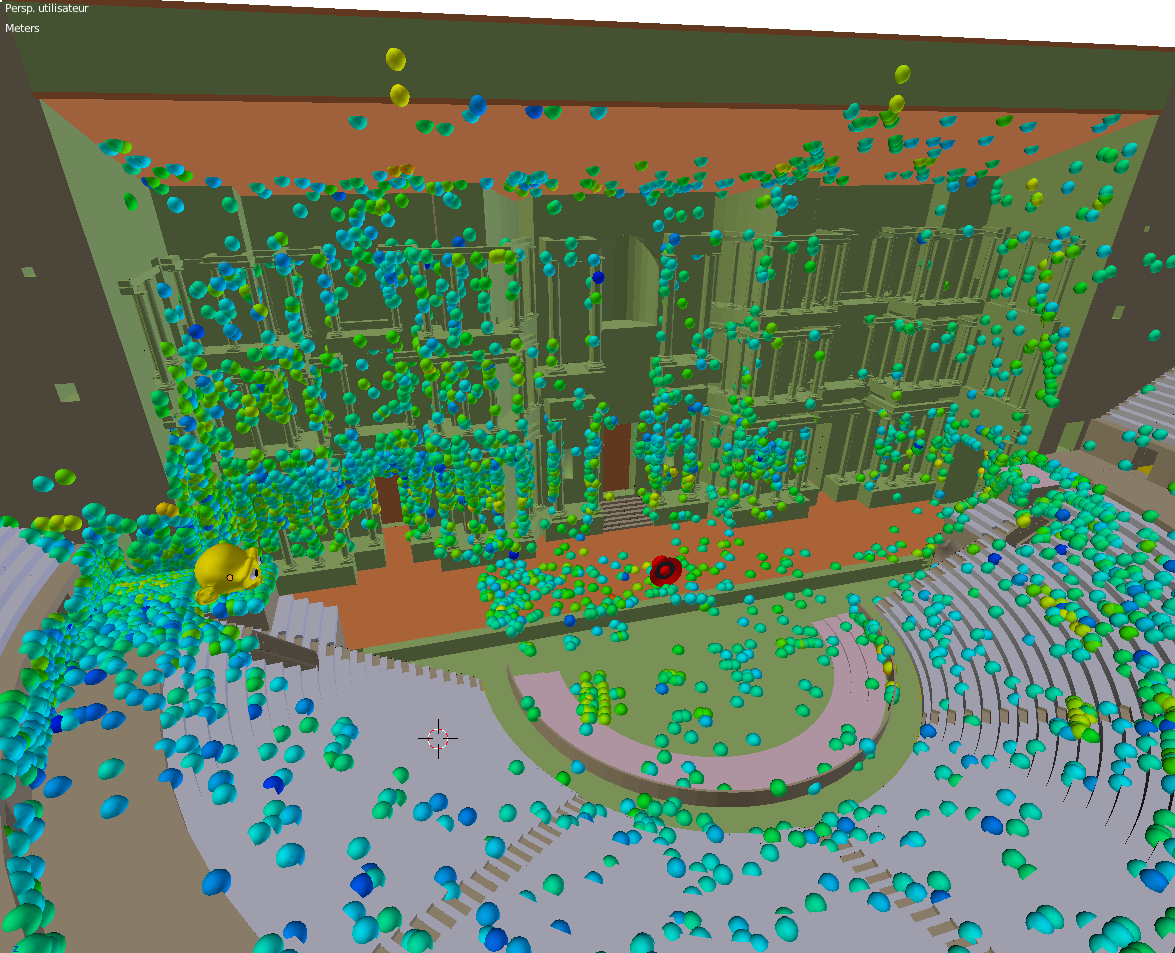
\includegraphics[width=\linewidth]{images/Listener10}
		\caption{Projection des sources-images pour un auditeur situé sur la tribune occidentale pour 1~000~000 de rayons.}
	\label{listener10}
\end{figureth}
%
%\begin{itemize}
%\item Pour l'axe perpendiculaire au mur de scène (récepteurs 1 à 4), la clarté (\gls{C80}) et la définition (\gls{D50}) restent bien adaptées à la transmission de la parole. Le temps de réverbération double entre les premiers et derniers gradins ce qui dégrade légèrement ces paramètres. Néanmoins, le temps central (\gls{Ts}) restant inférieur à 50ms, on conserve un phénomène d'échos faible.
%\item Le long de l'axe décalé de 55° (récepteurs 5 à 9), le temps central (\gls{Ts}) se décale beaucoup plus loin (jusqu'à 136ms pour les derniers gradins) ce qui implique une moins bonne compréhensibilité. En effet lorsque l'auditeur n'est pas bien dans l'axe, le signal se réfléchi sur les cotés de la \gls{cavea} (notamment sur les murs lisses tels que les \glspl{podium}) ce qui ajoute beaucoup de signal au champs diffus.  
%\item Dans le troisième axe (récepteurs 10 à 12) cet effet est encore amplifié puisque le son se réfléchi sur les \glspl{basilique}. Le temps de réverbération est plus important au niveau de la tribune car cet auditeur bénéficie de nombreuses réflexions sur le mur de scène que les auditeurs du deuxième et troisième \gls{maenianum} n'ont pas. On constate alors que sur cet axe, l'acoustique n'est plus vraiment adaptée à la parole mais plutôt à la musique.
%\end{itemize}
%Le paramètre \gls{LF80} (dB) n'apparait pas dans le tableau \ref{tab_fac_rec} car la valeur reste toujours très faible (<0,1dB) conséquence du fait que le son provenant de la scène est grandement majoritaire.

Pour résumer, les spectateurs les plus éloignés entendaient le son jusqu'à dix fois moins fort. Plus on se rapproche de la scène, plus l'acoustique est favorable à la parole tandis que lorsqu'on s'approche de l'axe des \glspl{aditus}, l'acoustique est plus favorable à la musique.

\section{La source et le mur de scène}

Au théâtre d'Orange, il est probable que les sources sonores étaient composées d'instruments tels que les orgues hydrauliques \cite[p.65]{rocconi} et les \gls{aulos} \cite[p.33]{rocconi} ou bien de la voix des acteurs \cite[]{voixRomain}. Ainsi, leur directionnalité serait plutôt orientée vers le public et non vers le mur de scène. La fonction du mur semble donc, dans un premier temps, être décorative et isolante. En effet, la structure complètement enclavante du théâtre coupe les spectateurs des bruits extérieurs. Par ailleurs, la décoration détaillée du front de scène apporte inévitablement un effet de diffusion des fréquences audibles. Néanmoins, on peut explorer l'impact de la forme caractéristique du mur de scène sur la réflexion du son. Cette dernière est liée à la position de la source sonore. La figure \ref{test_source1} montre les rayons se propageant vers le mur de scène et revenant vers les spectateurs (dans le plan à 1m60 au dessus de la scène) dans la configuration de référence sans décor. On constate que le mur autour de la porte centrale renvoi des rayons sur une partie des gradins. Les rayons aux extrémités de cette partie rectiligne reviennent avec un angle de 30° environ. D'autre part, l'\gls{exedre} curviligne ainsi que les baldaquins en saillie renvoient les rayons vers les tribunes. On constate donc que dans cette configuration, la réflexion sur le mur ne permet pas de couvrir l'ensemble des gradins. La diffusion apportée par la décoration sera donc essentielle pour diffuser le son à l'ensemble des spectateurs. Les trois autres figures montrent que les réflexions sur le mur couvrent l'ensemble des gradins et que certaines zones sont soumises à un effet de focalisation. La figure \ref{test_source2} représente les réflexions sur le mur pour une source située sur l'axe entre les portes latérales menant aux \glspl{parascaenium} c'est-à-dire à Y=9m. On constate dans ce cas que l'\gls{exedre} curviligne permet de concentrer une partie des rayons sur les extrémités de la \gls{cavea}. De la même manière, grâce aux figures \ref{test_source3} et \ref{test_source4}, on constate bien que plus on s'éloigne du bord de la scène, plus l'\gls{exedre} concentre les rayons vers l'axe central de la \gls{cavea}. On voit d'ailleurs sur la figure \ref{test_source4} que lorsque la source est sur l'escalier de la porte royale, (quasiment dans l'encadrement), les rayons reviennent de part et d'autre de l'escalier central de la \gls{cavea}. 

\begin{figureth}
	\begin{subfigureth}{0.48\textwidth}
		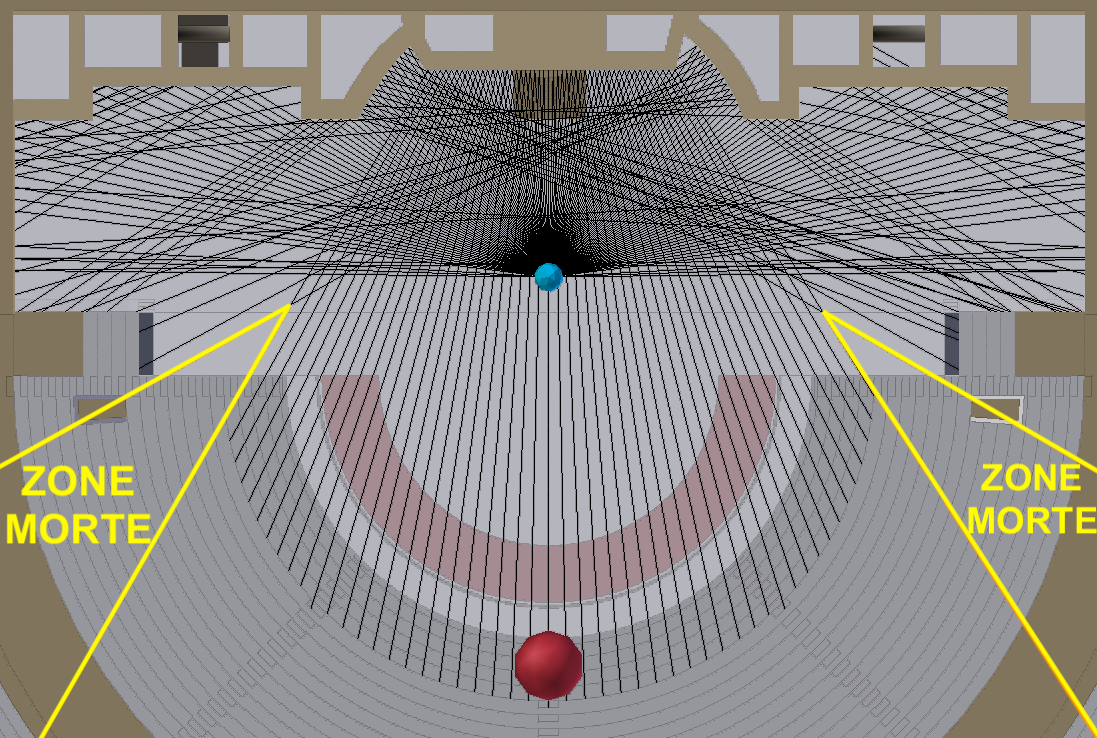
\includegraphics[width=\linewidth]{images/test_source1}
		\caption{Réflexions des rayons sur le mur de scène pour une source située en [0 ; 3,6 ; 42,8].}
		\label{test_source1}
		\hfill
		\quad
	\end{subfigureth}
	\quad
	\begin{subfigureth}{0.48\textwidth}
		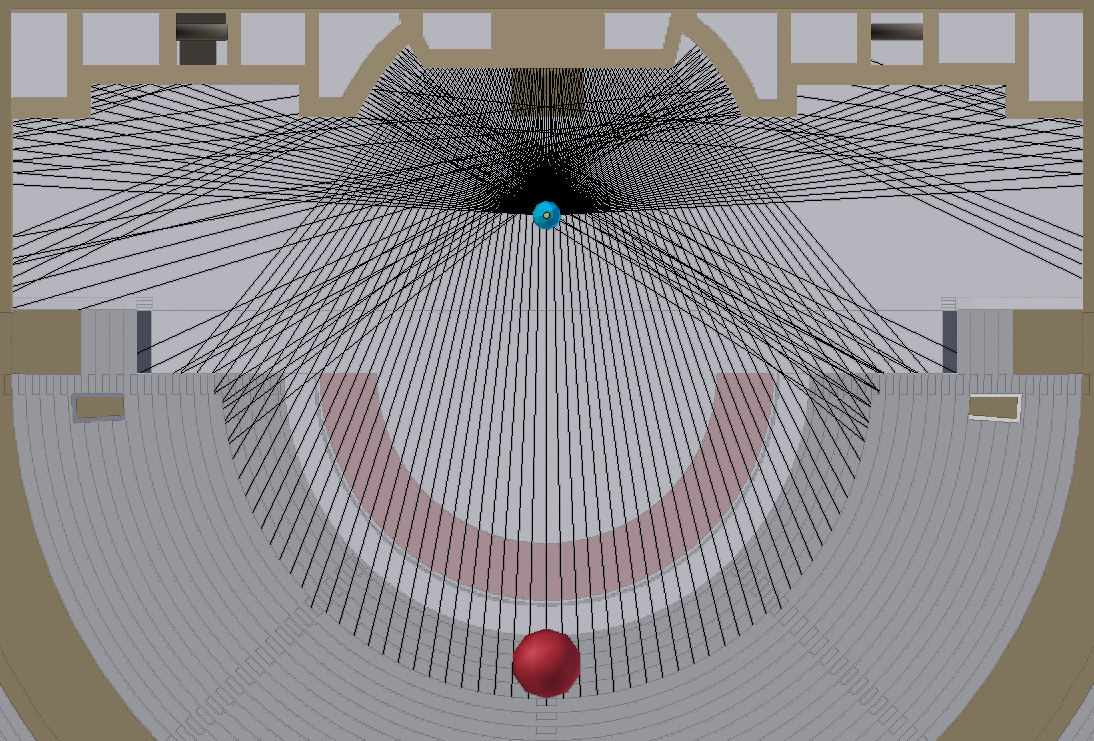
\includegraphics[width=\linewidth]{images/test_source2}
		\caption{Réflexions des rayons sur le mur de scène pour une source située en [0 ; 9 ; 42,8].}
		\label{test_source2}
		\quad
	\end{subfigureth} 
	\begin{subfigureth}{0.48\textwidth}
		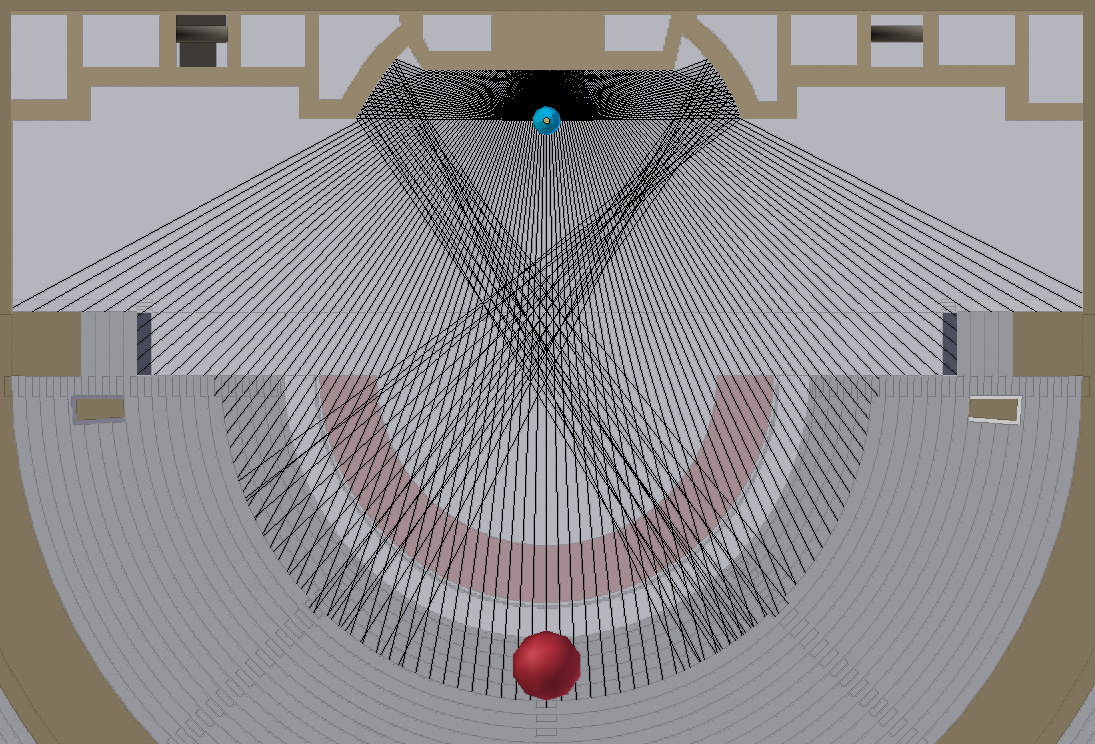
\includegraphics[width=\linewidth]{images/test_source3}
		\caption{Réflexions des rayons sur le mur de scène pour une source située en [0 ; 14,5 ; 42,8].}
		\label{test_source3}
	\end{subfigureth}
	\quad
	\begin{subfigureth}{0.48\textwidth}
		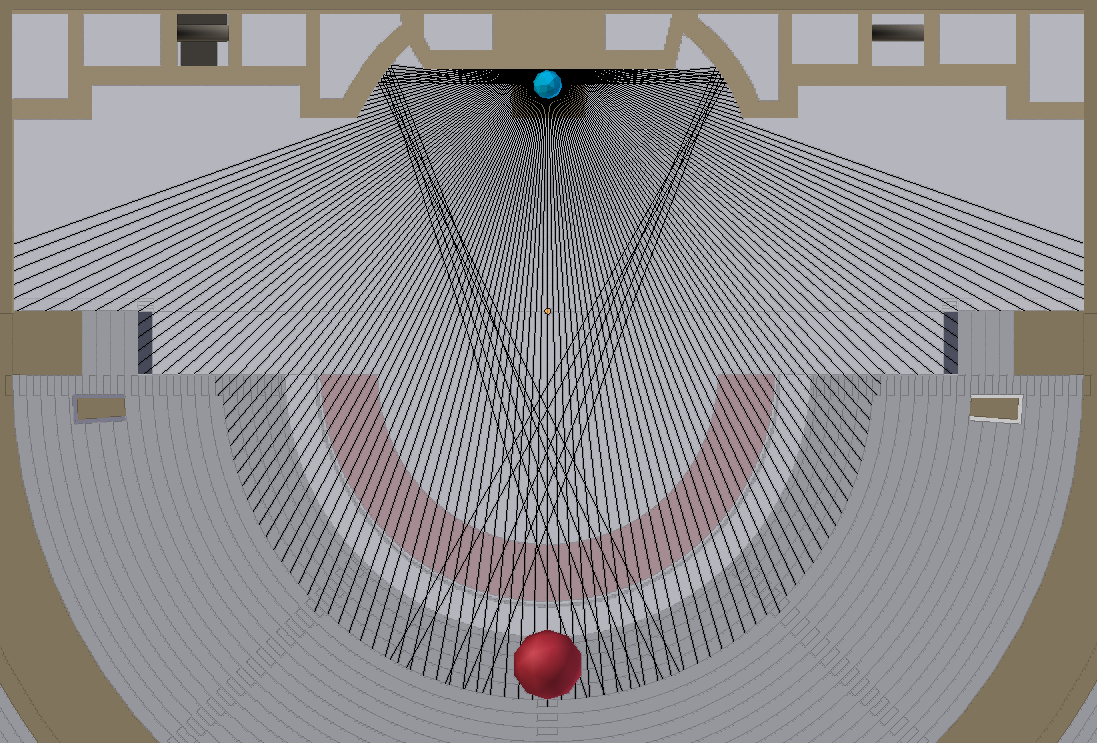
\includegraphics[width=\linewidth]{images/test_source4}
		\caption{Réflexions des rayons sur le mur de scène pour une source située en [0 ; 16,5 ; 42,8].}
		\label{test_source4}
	\end{subfigureth}
\caption{Réflexions des rayons propagés depuis une source vers le mur de scène dans un plan horizontal.}	
\label{test_source}
\end{figureth}	

Plaçons nous maintenant dans le plan vertical YZ (ou vu de profil). Nous avons vu précédemment que la réflexion sur l'orchestre est très importante puisqu'elle permet de renvoyer une grande partie des rayons vers les gradins. Cependant, plus la source va s'éloigner du bord de la scène, moins il y aura de rayons réfléchis sur l'orchestre. Les rayons sont alors réfléchis sur la scène qui possède des coefficients d'absorption plus élevés. On peut alors calculer la distance $d$ de l'orchestre qui va réfléchir des rayons en fonction de la distance $d'$ de la source sur la scène par rapport au bord (voir fig \ref{angle_refl}). D'après le théorème de Thalés on a :
\begin{equation}
d = \frac{h'}{h}\times d' = 1,33d',
\end{equation}
où :
\begin{itemize}
\item h est la hauteur de la scène (1,2m à Orange),
\item h' est la hauteur de la source sur la scène (1,6 m en prenant en compte la taille moyenne d'un acteur).
\end{itemize}
Ainsi, lorsque que l'acteur s'éloignera du bord de la scène de 1m, les réflexions se feront sur 1,33m de moins sur l'orchestre. On note par ailleurs que les escaliers de la porte royales se trouvent à 11m du bord de la scène ; lorsque l'acteur sera à cette position, les rayons ne toucheront l'orchestre qu'à 14,63m du bord de la scène, ce qui tombe en plein dans les gradins mobile. Un acteur se trouvant en fond de scène ne bénéficiera donc pas de la réflexion sur l'orchestre pour amplifier le son.
\begin{figureth}
	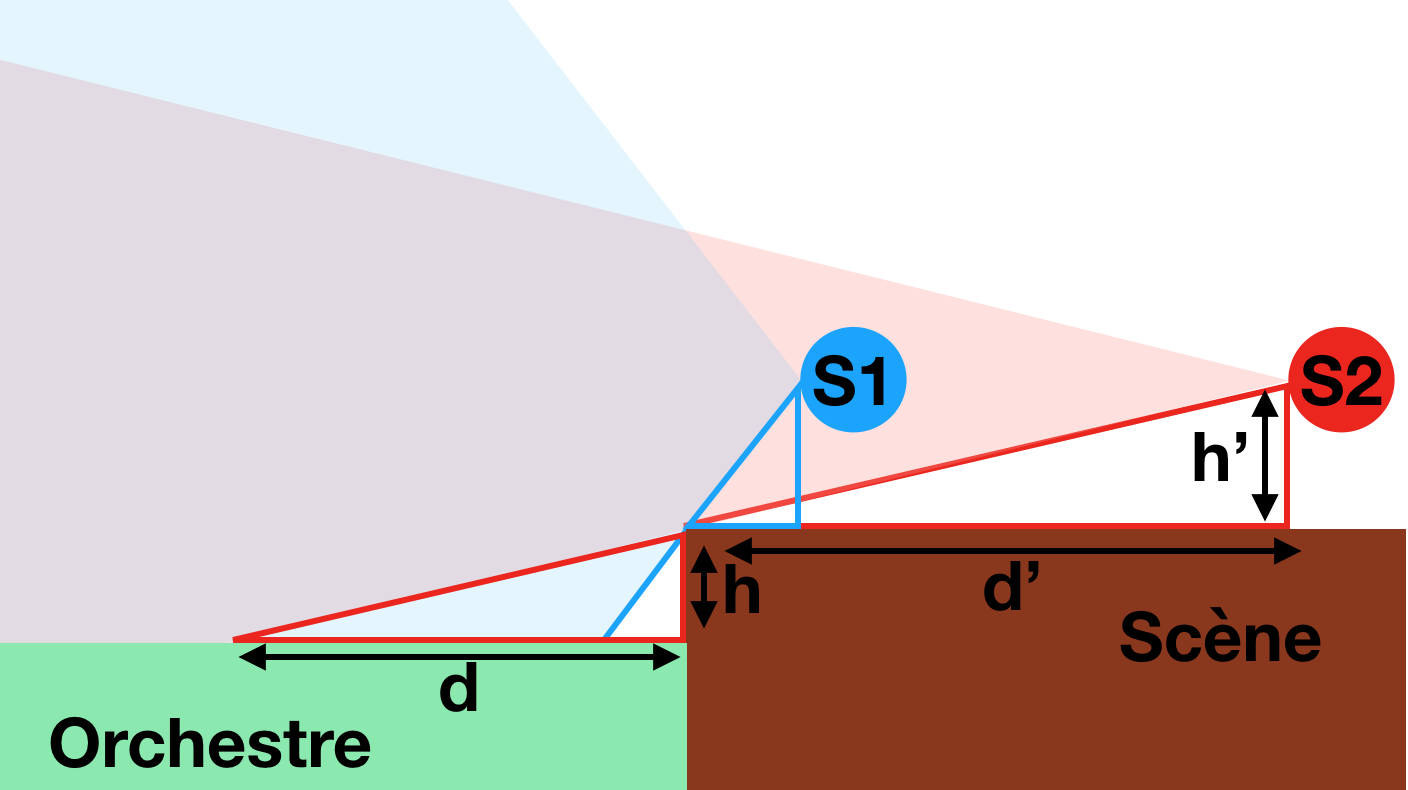
\includegraphics[width=0.8\linewidth]{images/angle_refl}
	\caption{Vu de profil de la propagation sonore à partir de deux sources S1 et S2. Proportion de signal réfléchi sur l'orchestre plus faible pour S2 que pour S1.}
	\label{angle_refl}
\end{figureth}


Nous plaçons maintenant la source au niveau de la porte latérale occidentale du mur de scène centrée dans la profondeur au niveau de l'axe entre les portes des deux \glspl{basilique}. On constate sur la figure \ref{RIR20sourcelat} qu'il y a quelques échos suffisamment espacés pour être discernés. Tout de suite après le son direct, la réflexion ne provient pas de l'orchestre mais des degrés bas munies de sièges mobiles. Celui-ci est donc fortement atténué et l'effet miroir de l'orchestre est perdu. Il pourra exister pour les spectateurs situés dans la partie orientale de la \gls{cavea} puisque l'angle le permettra. Le grand pic situé à 30ms environ après le son direct est lié aux réflexions sur les parties basses du mur de scène. Les pics d'énergie plus tardifs sont liés aux réflexions sur le toit.
%
\begin{figureth}
	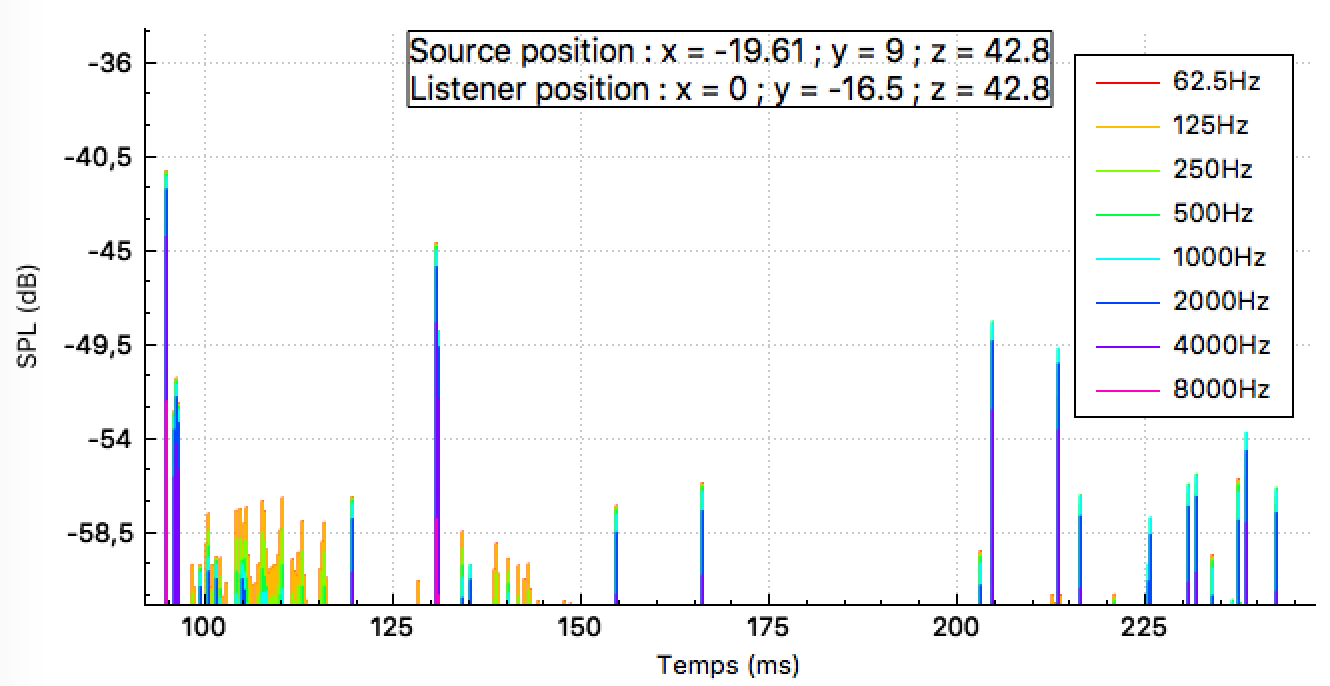
\includegraphics[width=0.7\linewidth]{images/RIR20sourcelat}
	\caption{Réponse impulsionnelle jusqu'à -20dB pour une source latérale située en [-19.61 ; 9 ; 42.8] et un récepteur en position initiale [0 ; -16.5 ; 42.8] pour 1000000 de rayons.}
	\label{RIR20sourcelat}
\end{figureth}
%
Le tableau \ref{tab_fac_rec_sourcelat} représente le temps de réverbération et les indices de compréhensibilité pour différentes positions de spectateurs (voir fig. \ref{sourcelat}). Les indices 6', 9', etc sont les récepteurs symétriques aux 6, 9, etc par rapport à l'axe central. Notons déjà qu'avec une source à cette position le gain est de 9dB environ donc 2dB de plus que dans la position initiale. Nous constatons alors que les spectateurs sur l'aile orientale ont une compréhensibilité médiocre tandis que ceux sur la tribune occidentale (récepteur 10) en ont une correcte. Le récepteur 12 ne peut pas être pris en compte en l'état car le son direct n'est pas perçu, les valeurs de clarté et définition sont donc faussées.

\begin{figureth}
	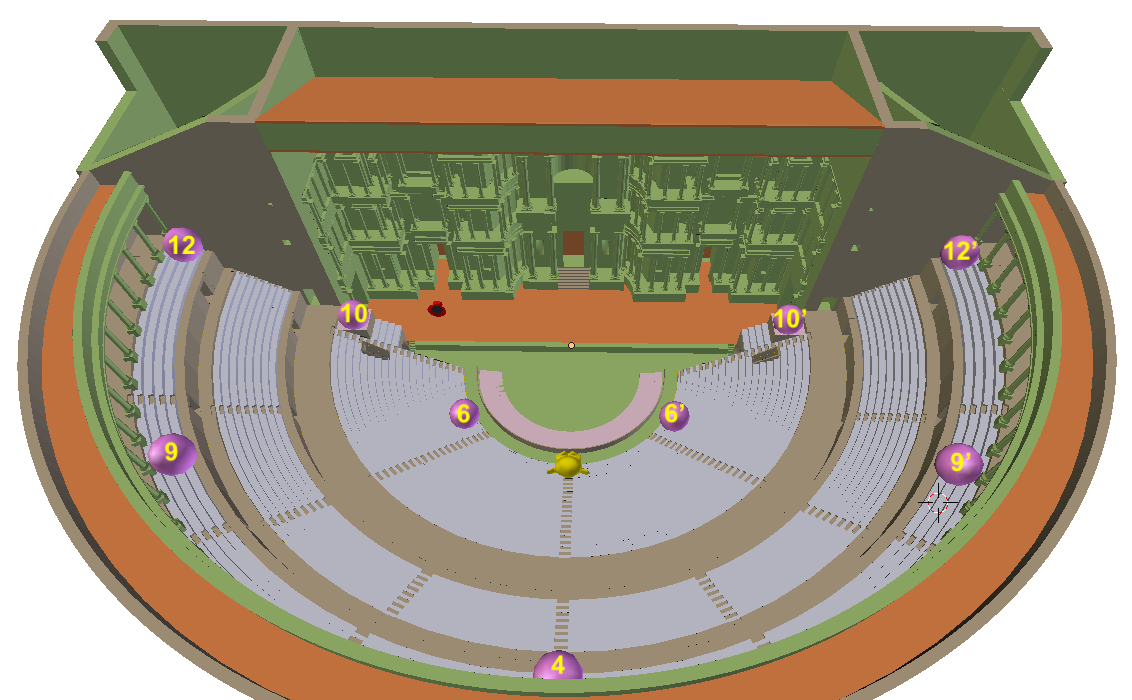
\includegraphics[width=0.9\linewidth]{images/sourcelat}
	\caption{Répartition des récepteurs pour le test de source latérale.}
	\label{sourcelat}
\end{figureth}

\begin{tableth} 
%\footnotesize
 \begin{tabular}{| *{9}{c|}} 
 \hline 
 Récepteur & [x ; y ; z] (m)  & \gls{T30} (ms) & \gls{C80} (dB) & \gls{D50} (\%)  \\ 
 \hline 
 \hline 
 Réf    &[0 ; -16.5 ; 42.8] &3710  &0.77  &51.22  \\
 \hline 
  4  &  [0 ; -44.36 ; 62.06] &4655  &1.2  &48.27  \\
 \hline 
 \hline
 6  &  [-13.51 ; -9.46 ; 43.86] &3685  &1.58  &54.82  \\%11
  \hline 
 9  & [-36.34 ; -25.44 ; 62.06] &4681  &0.9  &43.82  \\%8
 \hline 
 \hline
 10  &  [-28.23 ; 1.66 ; 50.02] &4548  &3.22  &55.73  \\%7
 \hline 
12   & [-44.36 ; 1.66 ; 62.06] &5518  &-14.23  &2.96  \\%5
 \hline  
 \hline
 6'  &  [13.51 ; -9.46 ; 43.86] &3597  &-0.01  &40.71  \\%3
  \hline 
 9'  & [36.34 ; -25.44 ; 62.06] &4635  &-1  &34.69  \\%19
 \hline 
 \hline
 10'  &  28.23 ; 1.66 ; 50.02] &4612  &-2.18  &22.98  \\
 \hline 
12'   & [44.36 ; 1.66 ; 62.06] &5362  &-6.49  &17.11  \\%0
 \hline 
\end{tabular} 
 \caption{Facteurs perceptifs pour différents récepteurs sur la bande de fréquence de 500Hz pour 1~000~000 de rayons et une source en [-19.61 ; 9 ; 42.8].} 
 \label{tab_fac_rec_sourcelat} 
 \end{tableth}

Nous avons vu précédemment que la niche centrale renvoie une partie du son émis par une source depuis la scène. Qu'en est-il d'une source qui serait située dans la niche même ? En étudiant le \gls{postscaenium}, notamment les différents passages permettant de circuler à l'intérieur du mur de scène, nous constatons que l'accès à cette grande niche centrale est praticable et qu'il existe des ouvertures pour y faire entrer des personnes. La figure \ref{voute} montre la trajectoire des rayons lorsque la source est située dans la niche. On constate que l'intégralité des gradins est couverte et qu'une partie du son se réfléchit sur le toit au dessus de scène pour mieux repartir vers la \gls{cavea}. Par ailleurs, le tableau \ref{tab_niche} montre que le gain est 6dB supérieur à la configuration de référence, l'énergie est donc quatre fois plus grande. On voit également que la compréhensibilité sera excellente car la définition est au delà de 70\%. Cet emplacement semble donc parfaitement convenir à l'émission de son, grâce au fait que celui-ci est amplifié par l'arrière de la niche qui présente une surface très réfléchissante. Cette niche voutée fonctionne donc exactement comme un porte-voix. On pourrait alors imaginer l'apparition de personnages divins \cite[p.12]{vitruve} avec une voix d'une puissance surdimensionnée et d'une grande clarté.
\begin{figureth}
	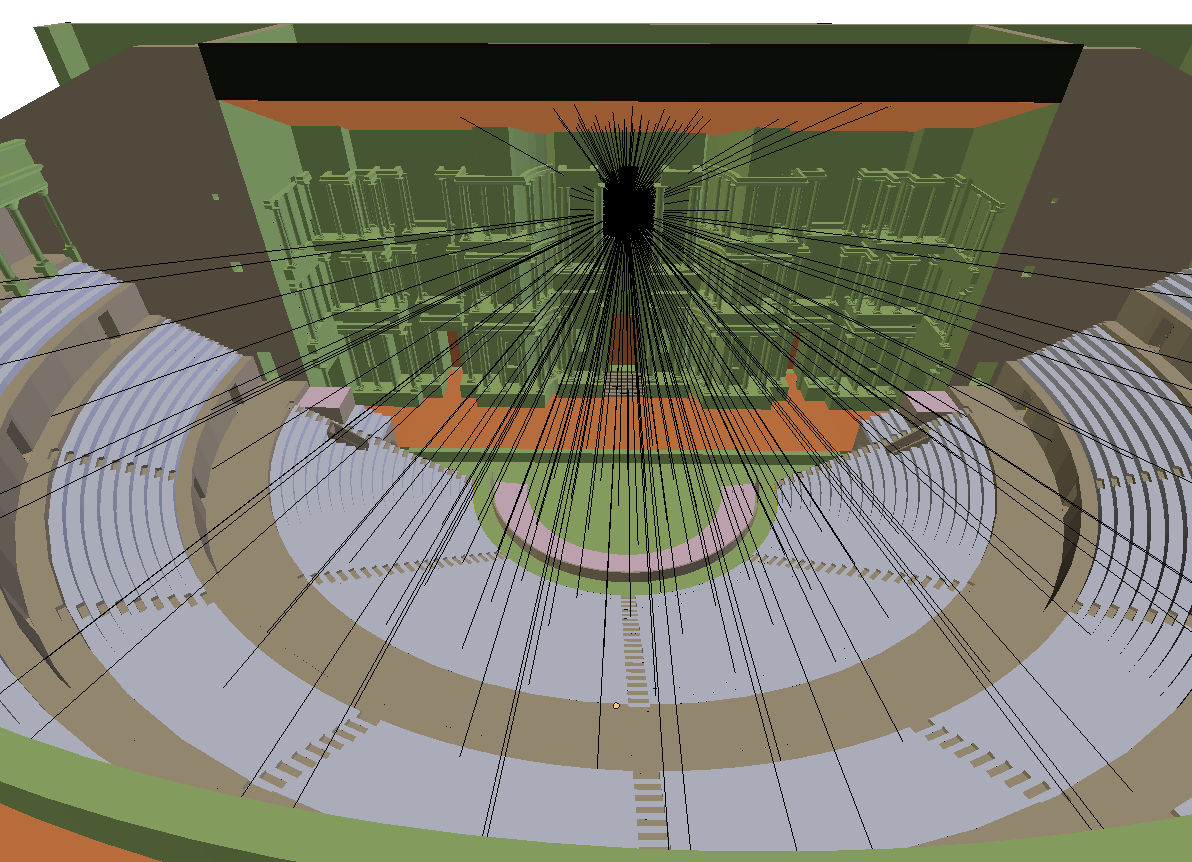
\includegraphics[width=0.8\linewidth]{images/voute}
	\caption{Propagation de 1000 rayons depuis la niche centrale.}
	\label{voute}
\end{figureth}

\begin{tableth} 
 \begin{tabular}{| *{9}{c|}} 
 \hline 
 Facteur & 62,5Hz & 125Hz & 250Hz & 500Hz & 1kHz & 2kHz & 4kHz & 8kHz \\ 
 \hline 
 \hline 
\gls{EDT} (ms)& 1890& 1857& 1553& 1147& 755& 714& 368& 171 \\ 
 \hline 
\gls{T30} (ms)& 4082& 3985& 3662& 3173& 2720& 2272& 1499& 628 \\ 
 \hline 
\gls{spl} (dB)& -29& -29& -30& -31& -31& -32& -36& -46 \\ 
 \hline 
\gls{G} (dB)& 13.7& 13.7& 13& 12.5& 12.2& 11.9& 11.4& 10.6 \\ 
 \hline 
\gls{C80} (dB)& 6.03& 6.08& 6.55& 6.9& 7.31& 8.24& 10.63& 16.2 \\ 
 \hline 
\gls{D50} (\%)& 71.96& 72.14& 74.9& 77.13& 78.95& 81.88& 87.48& 94.6 \\ 
 \hline 
\gls{Ts} (ms)& 88& 87& 74& 64& 57& 44& 27& 14 \\ 
 \hline 
\gls{LF80} (dB)& 0.039& 0.039& 0.038& 0.037& 0.037& 0.037& 0.036& 0.036 \\ 
 \hline 
\end{tabular} 
 \caption{Facteurs perceptifs pour une source en [0 ; 18.93 ; 60.89], un auditeur en [0 ; -16.5 ; 42.8] et 1000000 rayons.} 
 \label{tab_niche} 
 \end{tableth}
%\section{L e mur de scène}	

%on ajoute l'escalier central 

%qt mettre niveau en db pour le nom des source images rvb


\section{Présence de spectateurs}
La présence d'un public modifie le temps de réverbération des salles, ainsi selon qu'elle soit pleine ou vide, la salle ne "sonnera" pas de la même manière \cite[p.212]{jouhaneau}. Nous comparons alors les facteurs perceptifs préalablement établis dans la configuration initiale pour un théâtre plein (voir tab.\ref{tab_fact_init}), un théâtre vide et un théâtre rempli aléatoirement à 70\%. La source et le récepteur sont positionnés dans la configuration initiale (voir section \ref{sect_config_init}). Lorsque le théâtre est complètement vide, c'est-à-dire que le matériau de tous les gradins n'est plus de type "Audience" mais de type "Calcaire" (voir section \ref{sect_config_init}), on observe logiquement que le temps de réverbération augmente considérablement (voir tab.\ref{tab_fac_vide}). En effet, le public absorbe les ondes sonores tandis que le calcaire les réfléchis fortement. Le test est donc effectué pour deux millions de rayons afin de pouvoir mesurer la réverbération sur un temps plus long. Ces multiples réflexions impliquent une augmentation du gain et une dégradation de la compréhensibilité.

Dans un second temps, on affecte de manière aléatoire un matériaux de type "Audience" à 70\% des faces des gradins. On obtient alors les résultats présentés dans le tableau \ref{tab_fac_70}. Nous constatons que les facteurs perceptifs évoluent de manière proportionnelle au pourcentage de spectateurs dans le théâtre. Ainsi, plus il y aura de spectateurs, meilleure sera la clarté. 

\begin{tableth} 
 \begin{tabular}{| *{9}{c|}} 
 \hline 
 Facteur & 62,5Hz & 125Hz & 250Hz & 500Hz & 1kHz & 2kHz & 4kHz & 8kHz \\ 
 \hline 
 \hline 
\gls{EDT} (ms)& 5813& 5666& 5388& 5293& 4518& 2993& 1436& 594 \\ 
 \hline 
\gls{T30} (ms)& 7809& 7672& 7144& 7061& 6630& 4643& 2178& 810 \\ 
 \hline  
\gls{G} (dB)& 10& 10& 10& 10.1& 9.8& 8.9& 7.3& 5.2 \\ 
 \hline 
\gls{C80} (dB)& -2.92& -2.85& -2.87& -3.06& -2.65& -1.36& 1.38& 7.34 \\ 
 \hline 
\gls{D50} (\%)& 28.7& 29.01& 28.85& 27.9& 29.76& 35.97& 50.5& 78.09 \\ 
 \hline 
\gls{Ts} (ms)& 344& 336& 322& 321& 278& 187& 93& 29 \\ 
 \hline 
\end{tabular} 
 \caption{Facteurs perceptifs pour une source en [0 ; 5.6 ; 42.8] et un auditeur en [0 ; -16.5 ; 42.8] et 1000000 rayons dans le cas d'un théâtre vide.} 
 \label{tab_fac_vide} 
 \end{tableth}
 
 
 \begin{tableth} 
 \begin{tabular}{| *{9}{c|}} 
 \hline 
 Facteur & 62,5Hz & 125Hz & 250Hz & 500Hz & 1kHz & 2kHz & 4kHz & 8kHz \\ 
 \hline 
 \hline 
\gls{EDT} (ms)& 2726& 2681& 2375& 2209& 2030& 1688& 1244& 521 \\ 
 \hline 
\gls{T30} (ms)& 5647& 5565& 5206& 4794& 4193& 3032& 1657& 696 \\ 
 \hline 
\gls{G} (dB)& 8& 8& 7.7& 7.7& 7.4& 7& 6& 4.4 \\ 
 \hline 
\gls{C80} (dB)& -0.17& -0.13& 0.1& 0.14& 0.44& 1.29& 3.42& 9.16 \\ 
 \hline 
\gls{D50} (\%)& 41.67& 41.89& 42.84& 42.82& 44.33& 48.76& 59.79& 82.39 \\ 
 \hline 
\gls{Ts} (ms)& 171& 168& 154& 147& 134& 107& 65& 22 \\ 
 \hline 
\end{tabular} 
 \caption{Facteurs perceptifs pour une source en [0 ; 5.6 ; 42.8] et un auditeur en [0 ; -16.5 ; 42.8] et 2000000 rayons dans le cas d'un théâtre rempli à 70\%.} 
 \label{tab_fac_70} 
 \end{tableth}

\section{Les couvertures}
%\section{Impact du bruit extérieur}
Voyons dans un premier temps l'impact de la couverture de la scène. Ce plafond incliné de 19° est orienté vers le public et recouvre entièrement la scène. Il était a priori composé de caissons qui auraient apporté un effet de diffusion (voir fig. \ref{caisson_toit}). Cependant, n'ayant aucune donnée pour confirmer cette hypothèse, nous nous contentons d'utiliser un plafond lisse pour ne tester que sa pure réflexivité. La figure \ref{toit} montre que sur l'axe central les réflexions successives sur le mur et sur le plafond permettent de couvrir l'ensemble des gradins.
\begin{figureth}
	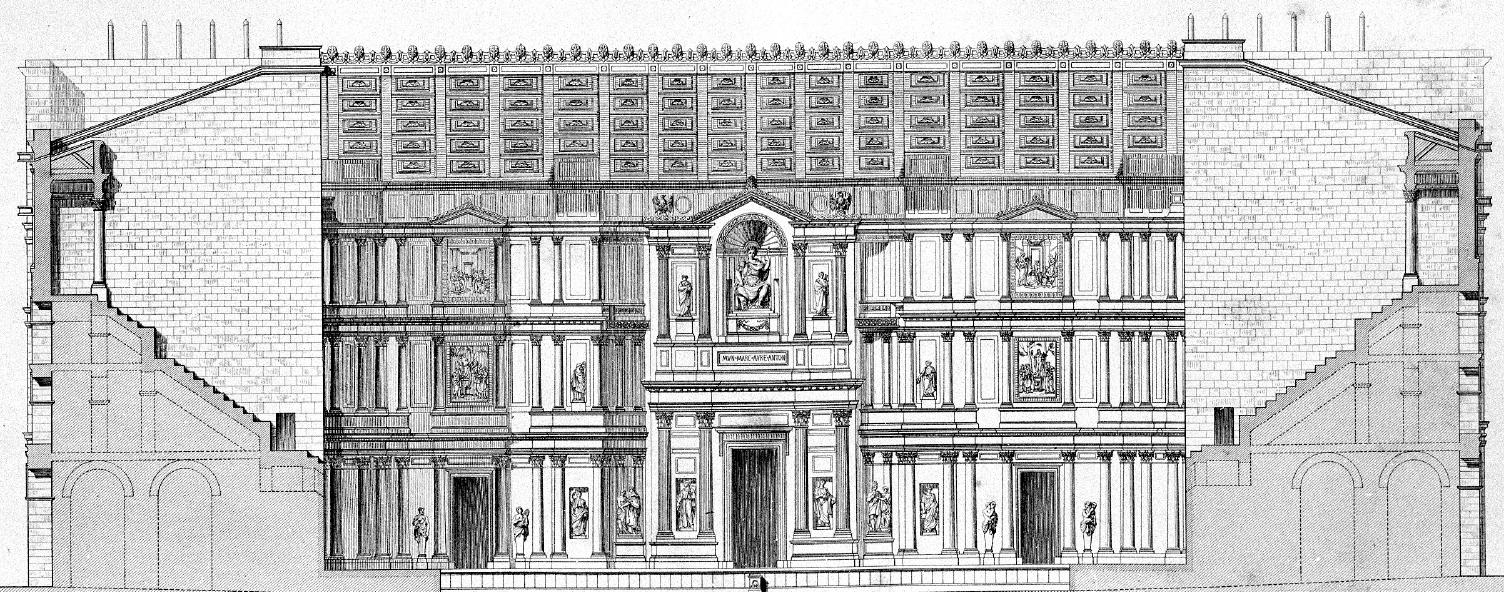
\includegraphics[width=\linewidth]{images/caisson_toit}
	\caption[Restitution du bâtiment de scène par A. Caristie représentant le plafond à caissons.]{Restitution du bâtiment de scène par A. Caristie représentant le plafond à caissons \footnotemark.}
	\label{caisson_toit}
\end{figureth}
\citefnt[Pl. III]{orangePl}
%
\begin{figureth}
	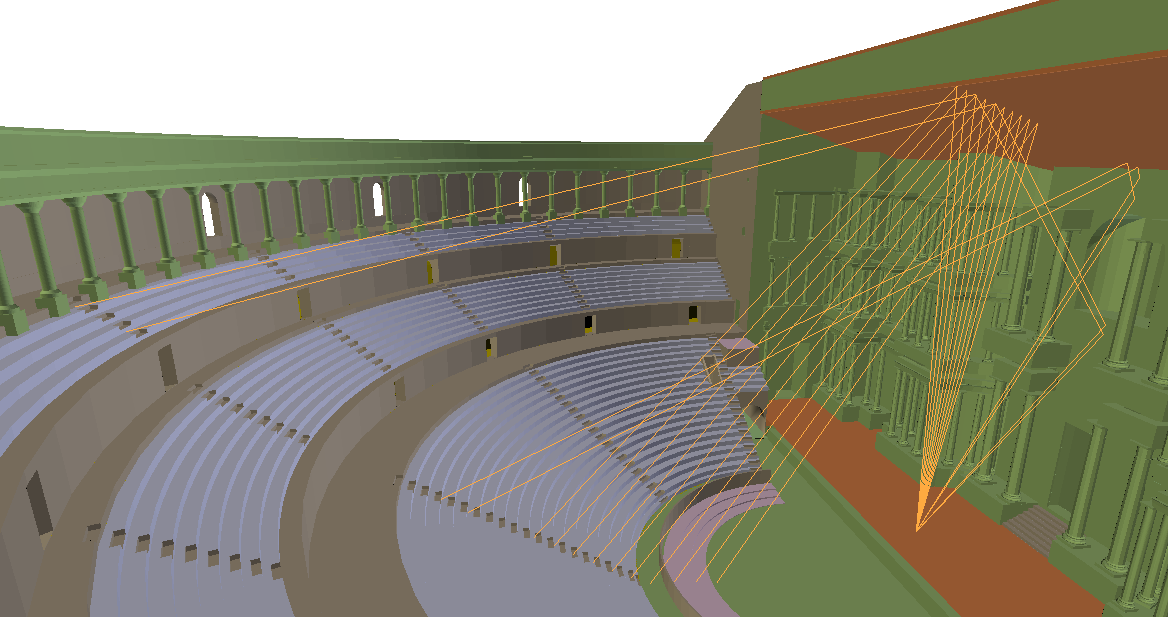
\includegraphics[width=\linewidth]{images/toit}
	\caption{Angle des rayons se propageant depuis l'avant scène et se réfléchissant successivement sur le mur de scène et sur le toit.}
	\label{toit}
\end{figureth}


Nous affichons la différence entre deux réponses impulsionnelles, avec et sans toit (voir fig \ref{diff_toit}). Nous constatons que le toit n'a d'impact que sur les premières réflexions et qu'il va générer principalement deux échos.
%
\begin{figureth}
	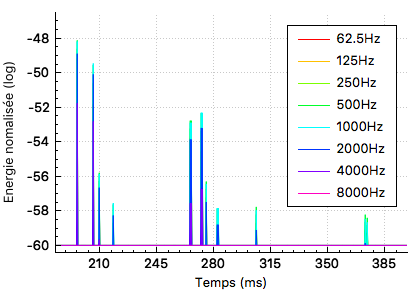
\includegraphics[width=0.6\linewidth]{images/diff_toit}
	\caption{Différence entre les réponses impulsionnelles avec et sans toit pour une source et un récepteur positionnés dans la configuration initiale pour 1~000~000 de rayons.}
	\label{diff_toit}
\end{figureth}
%
\begin{tableth}
 \begin{tabular}{| *{9}{c|}} 
 \hline 
 Facteur & 62,5Hz & 125Hz & 250Hz & 500Hz & 1kHz & 2kHz & 4kHz & 8kHz \\ 
 \hline 
 \hline 
\gls{EDT} (ms)& 1867& 1854& 1636& 1501& 1323& 1130& 623& 387 \\ 
 \hline 
\gls{T30} (ms)& 3417& 3416& 3211& 2966& 2700& 2218& 1383& 672 \\ 
 \hline 
\gls{G} (dB)& 6.4& 6.4& 5.9& 5.5& 5.3& 5& 4.4& 3.5 \\ 
 \hline 
\gls{C80} (dB)& 2.4& 2.43& 3.14& 3.65& 4.1& 4.99& 7.01& 12.22 \\ 
 \hline 
\gls{D50} (\%)& 53.78& 53.96& 56.75& 58.48& 60.3& 64.04& 72.12& 86.9 \\ 
 \hline 
\gls{Ts} (ms)& 106& 105& 89& 81& 73& 59& 37& 14 \\ 
 \hline 
\end{tabular} 
 \caption{Facteurs perceptifs pour une source en [0 ; 5.6 ; 42.8] et un auditeur en [0 ; -16.5 ; 42.8] et 1000000 rayons sans plafond au dessus de la scène.}
 \label{tab_fact_sansToit} 
 \end{tableth}
 
 Le tableau \ref{tab_fact_sansToit} permet de comparer les facteurs perceptifs avec la configuration initiale. On constate que retirer le toit diminue le temps de réverbération et améliore la compréhensibilité. Cela se comprend aisément par la présence d'échos comme nous l'avons vu dans la section \ref{sect_analyse_rir}. On constate grâce au tableau \ref{tab_fac_listener_sansToit} que cela est vrai quelle que soit la position du spectateur (voir section \ref{sect_positionSpectateur}). Par ailleurs, le gain (donc le niveau sonore global) augmente de près d'1dB grâce à la présence du toit. 
 
 

On peut supposer que la \gls{porticus isc} avait un rôle similaire aux balcons des théâtres modernes, c'est-à-dire de rabattre le son sur les spectateurs. Les connaisseurs savent donc que les meilleures places en terme d'acoustique ne sont pas forcement les plus chères mais souvent celles situées sous les balcons car le son s'y réfléchit. Si cette astuce peut fonctionner pour la musique, elle produira l'effet inverse pour la parole puisque le temps de réverbération se trouve augmenté. Ainsi les spectateurs situés au niveau du troisième \gls{maenianum} seront privilégiés pour l'écoute musicale et lésés pour le texte. Même si la fonction première de la \gls{porticus isc} devait plutôt être pratique et esthétique, Vitruve explique que sa position doit également servir à l'acoustique : "la voix, en s'étendant, parviendra jusqu'à l'extrémité des degrés et jusqu'au haut de ce plafond" \cite[p.11]{vitruve}. La figure \ref{listener4} confirme que les spectateurs situés au sommet de la \gls{cavea} bénéficient principalement des réflexions sur la \gls{porticus isc}.
\begin{figureth}
	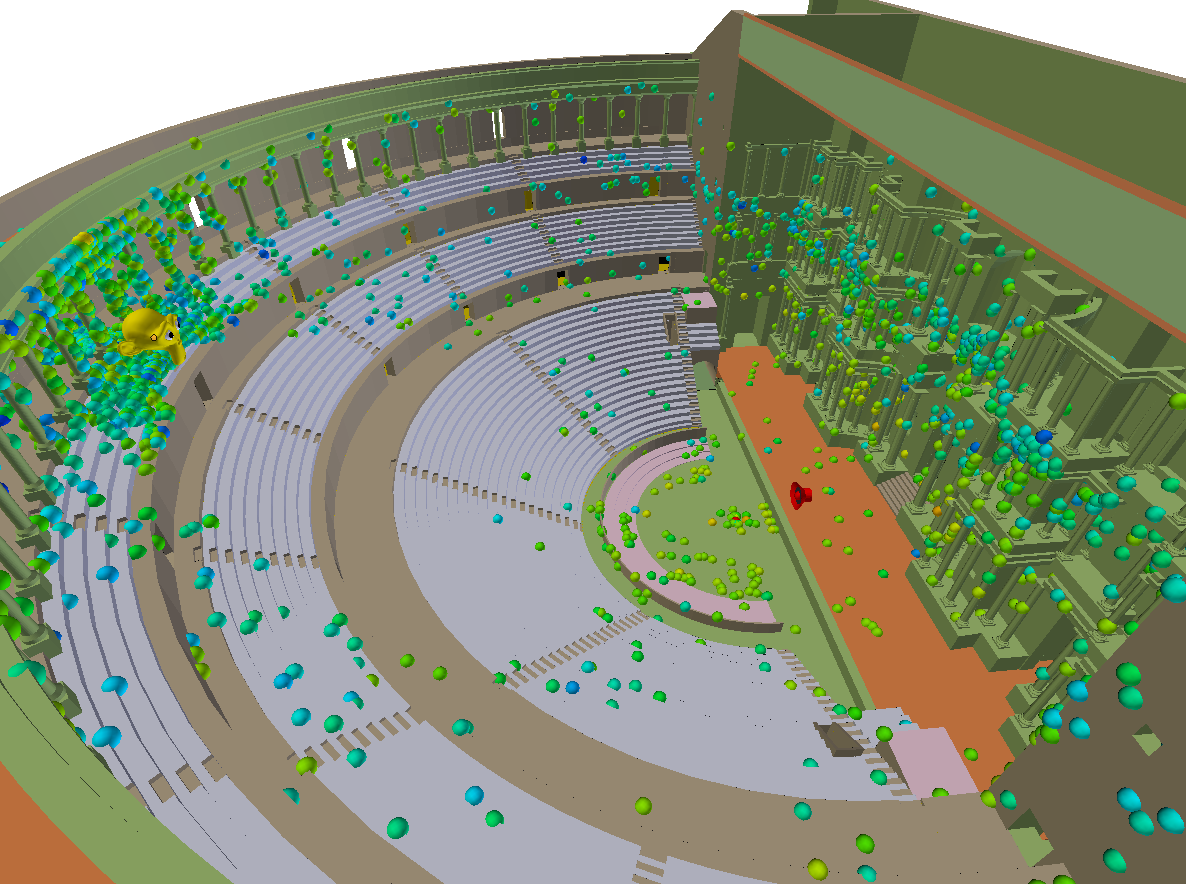
\includegraphics[width=0.8\linewidth]{images/Listener4}
	\caption{Projection des sources-images pour un auditeur situé sur le troisième \gls{maenianum} au niveau de l'axe central pour 1~000~000 de rayons.}
	\label{listener4}
\end{figureth}

Le \gls{velum} était a priori composé de toiles de lin \cite[p.38]{formige} suspendues au dessus de la \gls{cavea}. Ce type de matériau est très difficile à trouver dans les bases de données modernes car cet agencement est rare. Par ailleurs les tests sur tissus fait en laboratoire sont souvent effectués devant une surface dure. Or, dans notre cas, il n'y a aucune surface dure derrière les \glspl{velum}. Comment connaitre les coefficients d'absorption adéquats ? Nous savons que l'absorption d'un matériau est liée à sa porosité et sa fibrosité. En effet, si l'onde sonore peut pénétrer à l'intérieur du matériau, elle y engendre des frottements et des déplacements de fibres légères, d'où la transformation d'énergie. Ainsi, le tissu absorbe beaucoup les hautes fréquences et transmet les basses fréquences. \cite[Matériaux]{acouphile}. N'ayant pas plus d'information à ce sujet, nous considérons donc que très peu de son sera réfléchi sur le \gls{velum}. Ainsi les résultats établis avec et sans \gls{velum} seront très similaires. On peut néanmoins noter deux choses. Un \gls{velum} déployé peut permettre d'isoler des bruits extérieurs (hautes fréquences) au dessus du théâtre. Ils sont a priori très peu nombreux car il s'agirait du bruit des oiseaux ou du vent dans les arbres. Par contre, les voiles pourraient elles-mêmes être génératrice de bruit lorsque le vent s'y engouffre.
%\begin{tableth}
% \begin{tabular}{| *{7}{c|}} 
% \hline 
% Matériau & 125Hz & 250Hz & 500Hz & 1kHz & 2kHz & 4kHz \\ 
% \hline 
% \hline 
%Laine de lin \footnotemark & 0.09& 0.18& 0.48& 0.73& 0.50& 0.33 \\ 
% \hline 
%Moleton tendu \footnotemark & 0.50& 0.57& 0.48& 0.35& 0.28& 0.20 \\ 
% \hline 
%\end{tabular} 
% \caption{Matériaux pouvant être utilisés pour le \gls{velum}.}
% \label{tab_matVelum} 
% \end{tableth}


\section{Comparaison avec d'autres théâtres antiques} \label{sect_comptheatre}
Ces analyses permettent de comparer le théâtre d'Orange avec d'autres monuments similaires. Cela a déjà été entrepris par F. Canac par exemple lors de mesures \textit{in situ} (voir fig. \ref{canac_comparaison}). Notons que sur ce graphique l'échelle des abscisses de Orange et Aspendos a été décalée par rapport à celle d'Epidaure pour faciliter la lecture. Cette étude \cite[137-162]{canac} révèle que, dans leur état moderne, les théâtres d'Aspendos (Turquie), d'Orange et d'Epidaure (Grèce) peuvent se classer dans cet ordre si l'on compare leur gain (c'est-à-dire l'intensité sonore à égale distance pour une source de niveau identique). Cela est directement lié au pourcentage d'ouverture du théâtre. Ainsi, Aspendos étant le théâtre le plus cloisonné des trois, c'est celui qui aura le plus fort gain. Par ailleurs, on constate que dans les trois cas, l'onde parcours l'ensemble des gradins sans obstacle puisque la décroissance n'est dû qu'à la distance et que les trois courbes sont parallèles.
%
\begin{figureth}
	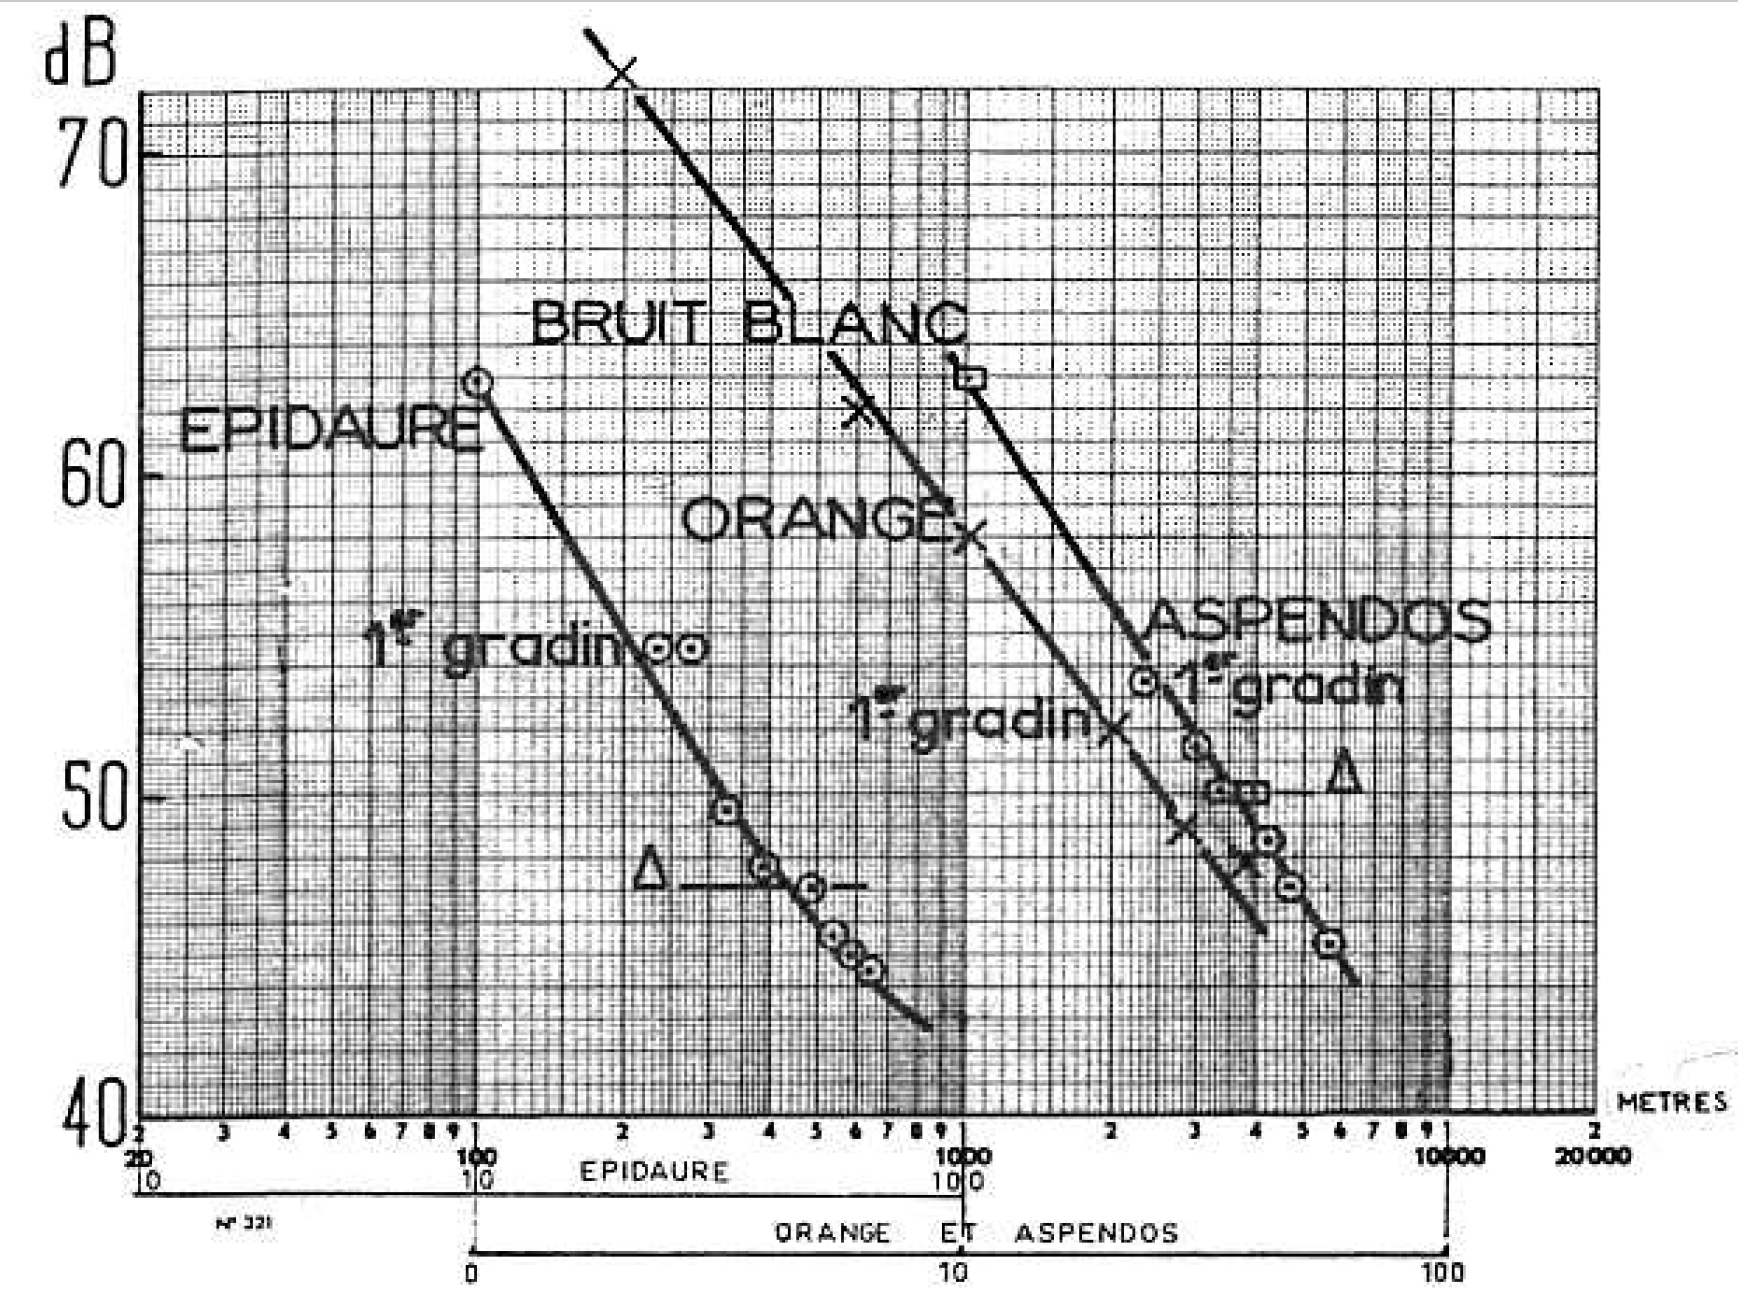
\includegraphics[width=0.7\linewidth]{images/canac_comparaison}
	\caption[Comparaison de l'intensité perçue entre les théâtre d'Epidaure, Aspendos et Orange.]{Comparaison de l'intensité perçue entre les théâtre d'Epidaure, Aspendos et Orange \footnotemark.}
	\label{canac_comparaison}
\end{figureth}
\citefnt[p.162]{canac}


Le problème de ce genre d'analyse est qu'on ne tient pas compte de l'apparence initiale des théâtres. Seules des maquettes le permettent et en l'occurence les maquettes virtuelles. On citera comme exemple le projet ERATO \cite{rindel} qui vise à comparer virtuellement les restitutions des théâtres d'Aspendos, de Jerash (Jordanie), de Syracuse (Sicile) ainsi que les \glspl{odeon} d'Aosta (Italie) et d'Aphrodisia (Turquie). Ces monuments sont testés sur le logiciel \textit{Odeon} (voir fig. \ref{rindel}). L'étude confirme que, comme pour le théâtre d'Orange, la gain d'un théâtre vide est plus important et la clarté est plus faible qu'avec un théâtre plein. Néanmoins, comme nous l'avons montré tout au long de cette partie, les résultats sont très dépendants de la configuration du théâtre ainsi que de la position des sources et récepteurs. Pour commencer, en complément de la section \ref{sect_val_odeon}, nous vérifions si dans le cas du théâtre d'Orange les résultats obtenus sur notre logiciel et sur \textit{Odeon} sont identiques. Le tableau \ref{tab_rindel} montre que les résultats sont effectivement sensiblement similaires. Notons que le chargement du maillage du théâtre d'Orange (environ 160~000 éléments) se fait en 20min sur \textit{Odeon}. Le calcul à -60dB pour 1~000~000 de rayons se fait ensuite en 6min. Notre logiciel exécute l'ensemble de la chaine en 8min. Nous rappelons une nouvelle fois que nous configurons \textit{Odeon} avec des options de paramétrage standard qui pourraient peut-être être mieux choisies.

Si on compare maintenant nos résultats avec ceux du projet ERATO, on constate qu'il est difficile de conclure (voir tab.\ref{tab_rindel2}). On pourrait comprendre que le théâtre d'Orange a un temps de réverbération plus long que les autres monuments et une mauvaise clarté (seule l'\gls{odeon} d'Aosta a une clarté inférieure) mais cela suppose que les configuration soient vraiment parfaitement comparables. En effet, le niveau de restitution des théâtres, le choix des matériaux et les positions des sources et des récepteurs peuvent engendrer des écarts d'un bâtiment à l'autre faussant la comparaison. Il semble donc que la meilleure démarche pour qualifier l'acoustique d'un monument antique soit de procéder comme nous l'avons fait, c'est-à-dire de manière relative sur une seule et même maquette. Pour comparer plusieurs théâtres entre eux il semble indispensable d'opérer soi-même les simulations pour être sûr de maitriser tous les paramètres. 
%
\begin{figureth}
	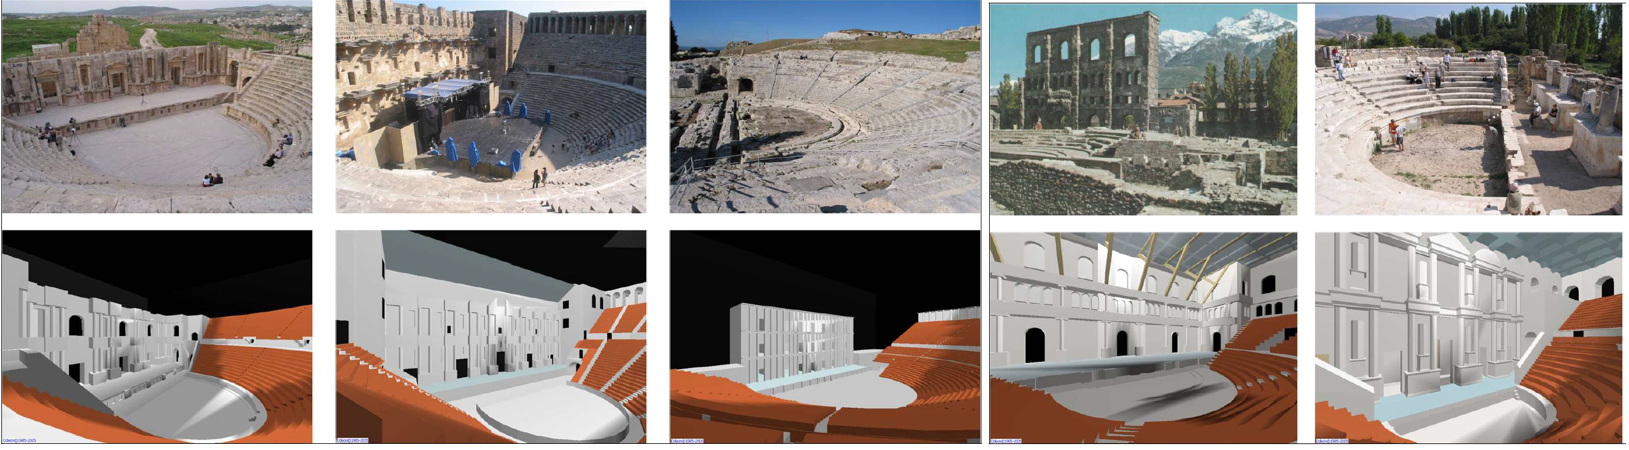
\includegraphics[width=\linewidth]{images/rindel}
	\caption[Photos des monuments sélectionnés et leur modèle virtuel restitué par le projet ERATO.]{Photos des monuments sélectionnés et leur modèle virtuel restitué par le projet ERATO \footnotemark. De gauche à droite : Jerash, Aspendos, Syracuse, Aosta, Aphrodisia.}
	\label{rindel}
\end{figureth}
\citefnt[fig.1 et 2]{rindel}
%
\begin{tableth}
 \begin{tabular}{| *{3}{c|}} 
 \hline 
 Facteur & Orange & Orange (via \textit{Odeon})   \\ 
 \hline 
 \hline 
  \gls{EDT} (s)& 1.85& 2.1 \\ 
 \hline 
\gls{T30} (s)& 3.59&  2.73\\ 
 \hline 
\gls{spl} (dB) &-32 & -32.4\\ 
 \hline 
\gls{C80} (dB)& 1.12&1.5  \\ 
 \hline 
\gls{D50} (\%)&47 & 52 \\ 
 \hline 
\gls{Ts} (ms)&117 & 105 \\ 
 \hline 
\end{tabular} 
 \caption{Comparaison des facteurs perceptifs du théâtre d'Orange déterminés dans notre étude en configuration de référence avec ceux simulés sur le logiciel \textit{Odeon} sur la bande de fréquence 500-1000Hz.}
 \label{tab_rindel} 
 \end{tableth}
 
 \begin{tableth}
 \begin{tabular}{| *{4}{c|}} 
 \hline 
 Monument & \gls{T30} (s) & \gls{spl} (dB) & \gls{C80} (dB)  \\ 
% Monument & \gls{EDT} (s) & \gls{T30} (s) & \gls{C80} (dB)  \\ 
 \hline 
 \hline 
Orange (sans décor) & 3.8  & -32   &  1      \\ 
%Orange (sans décor) & 0.8 & 2.7  & 5.4       \\ 
  \hline
Jerash & 1  & -34 & 6.9  \\ 
%Jerash & 0.45  & 0.81  & 11  \\ 
  \hline 
Aspendos & 1.6 & -35.4  & 4  \\ 
%Aspendos & 0.95 & 1.3  & 9  \\ 
 \hline 
Syracuse & 1.7  & -39  & 8.2  \\ 
%Syracuse & 0.28  & 1.29  & 13.5  \\ 
 \hline 
Aosta & 3.49  & -26.7  & -2.4     \\
%Aosta & 2.41  & 2.17  & 2.5     \\ 
 \hline 
Aphrodisia & 1.6  & -25  & 1.8     \\ 
%Aphrodisia & 1.64  & 1.78  & 3.7     \\  
 \hline 
\end{tabular} 
 \caption{Moyenne des facteurs perceptifs de différents bâtiments antiques pour une source positionnée au centre à l'avant scène et plusieurs récepteurs situés sur un axe à 55°. Le test est effectué pour un théâtre plein et un million de rayons sur la bande de fréquence 500-1000Hz.}
 \label{tab_rindel2} 
 \end{tableth}


\newpage

%\chapter{Comparaison avec d'autres théâtres antiques}
%\citationChap{
%Si on veut connaitre un peuple, il faut écouter sa musique
%}{Platon}
%\minitoc
%\newpage
%
%Nous terminons cette partie par la présentation de quelques résultats acoustiques établis sur d'autres théâtres antiques. Ceux-ci proviennent de sources extérieures et nous les corrélerons avec les résultats issus de notre étude. Comment se situe le théâtre d'Orange par rapport aux autres théâtres dont l'excellent état de conservation permet l'étude ? 
%
%Dans ce chapitre nous verrons les cas de deux théâtres significatifs : Aspendos et Epidaure.
%
%\section{Aspendos}
%\section{Epidaure}
%\section{Autres cas}
%
%Citer  \cite[p.25]{rindel}
%
%
%%
%\begin{figureth}
%	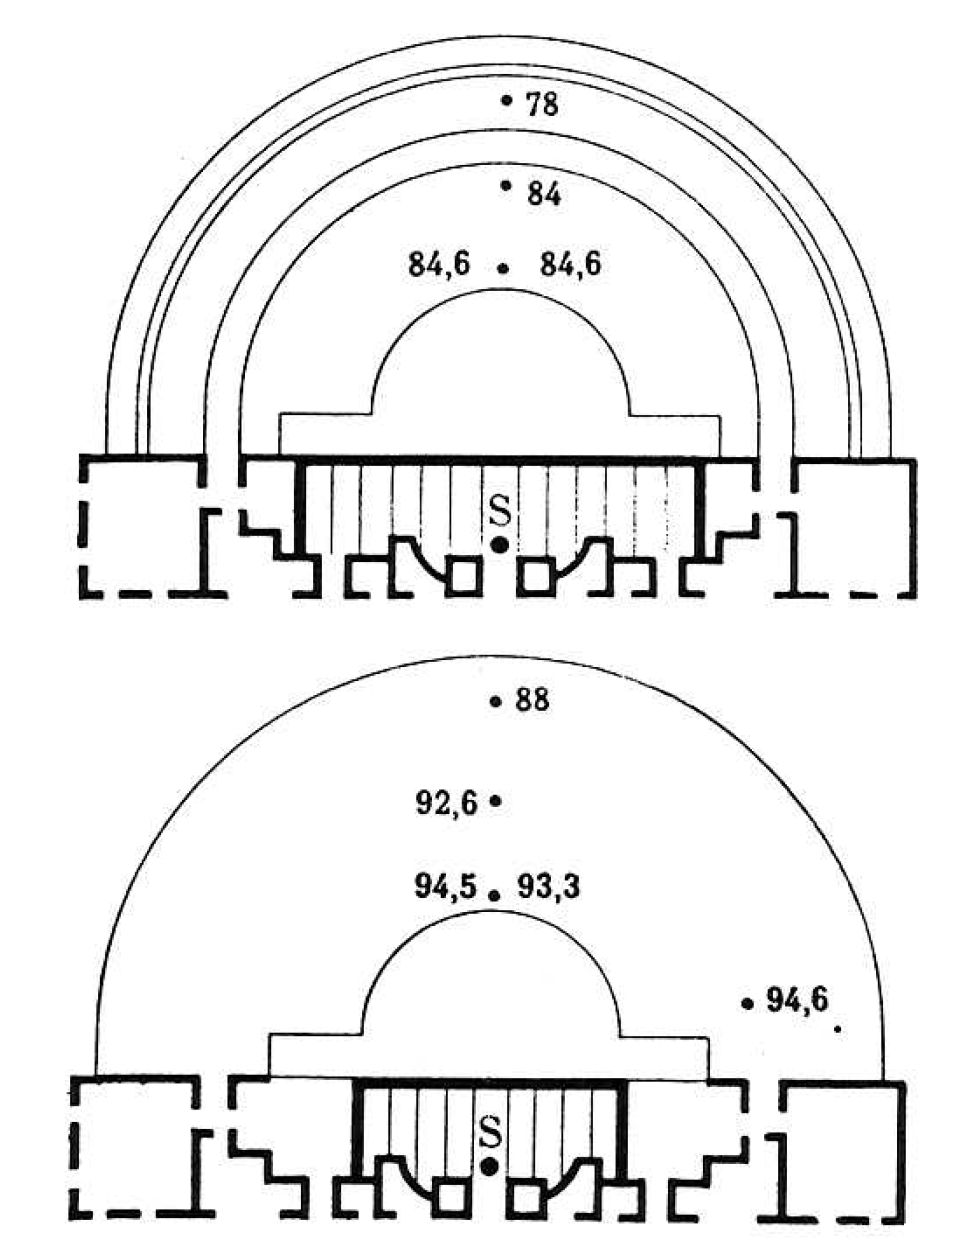
\includegraphics[width=0.7\linewidth]{images/canac_comparaison2}
%	\caption[Comparaison de la compréhensibilité à Orange, avec un mur (en haut) et à Vaison, sans mur (en bas).]{Comparaison de la compréhensibilité à Orange, avec un mur (en haut) et à Vaison, sans mur (en bas) \footnotemark.}
%	\label{canac_comparaison2}
%\end{figureth}
%\citefnt[p.152]{canac}



\chapter*{Conclusion}
\addcontentsline{toc}{chapter}{Conclusion}
Nous avons vu dans cette partie que la maquette virtuelle du théâtre d'Orange ainsi que l'outil de calcul acoustique développé durant ce projet permettent d'obtenir un certain nombre de résultats d'analyse. Comme nous l'avons vu, l'acoustique de ce bâtiment a été maintes fois discutée et étudiée mais, à notre connaissance, aucune étude ne s'est portée sur le théâtre à ce niveau de restitution. Nous avons ainsi pu constater que le théâtre, de part son encloisonnement et ses matériaux très réfléchissant, amplifie le son émis depuis la scène. L'absence de plafond au dessus des spectateurs permet d'obtenir un niveau de compréhensibilité correct mais pas excellent. On comprend que la diction et la puissance vocale des acteurs seront deux éléments primordiaux pour être compris en tout point des gradins. La diction, car il est essentiel de bien séparer chaque syllabe afin de comprendre les mots, or, une forte réverbération allonge leur durée. Les spectateurs les plus loin de la scène ou ceux sur les ailes de la \gls{cavea} auront plus de mal à les distinguer et donc à bien percevoir le discours. La puissance sonore, car celle-ci diminue rapidement lorsqu'on s'éloigne de la source. Les dimensions du lieu étant gigantesques, il faut pouvoir maintenir un niveau sonore suffisant sur de grandes distances. Les spectateurs du dernier \gls{maenianum} bénéficieront néanmoins des réflexions sur le plafond de la \gls{porticus isc}. Nous avons vu par ailleurs que le \gls{velum} aurait peu d'effet sur l'acoustique et que le toit au dessus de la scène permet de renvoyer les ondes sonores sur l'ensemble du public. Cependant, ce dernier crée également des échos, ce qui dégrade la clarté vocale. Le décor du front de scène, quant à lui, diffuse une partie du son qui s'y réfléchit, ce qui dégrade également la clarté. A contrario, un son plus diffus et plus réverbéré sera plus agréable pour une écoute musicale. On imagine donc que la musique avait une place importante dans les spectacles tandis que la transmission de la parole était compensée par une excellente diction de la part des acteurs. Par ailleurs, nous avons vu qu'une source sonore placée dans la niche voutée centrale pouvait projeter le son à tous les spectateurs avec une puissance augmentée. Cela nous laisse imaginer la présence de personnages ou de bruitages spectaculaires à cet endroit. Nous avons également montré que, plus il y a de spectateurs, plus la voix de l'acteur est claire, par contre, l'effet d'amplification liée à l'architecture du bâtiment est réduit.


Dans le futur il sera alors extrêmement intéressant de mener des tests similaires avec des sources directionnelles. Nous prévoyons en outre, avant la fin du projet, d'enregistrer les instruments de musique antiques ainsi que des textes anciens en chambre sourde. Cela permettra d'écouter des sons similaires à ceux qui étaient émis sur la scène du théâtre d'Orange lors de sa période d'activité avec une réverbération proche qui celle qui "résonnait" dans ce lieu. Par ailleurs, l'oeuvre de Vitruve sur l'acoustique des théâtres antiques \cite[Livre V]{vitruve} laisse à penser que les architectes de l'époque avaient pensé à des configurations ayant des effets plus subtils. Vitruve traite pendant un chapitre entier de l'utilisation des harmonies pour améliorer le son des théâtres : " de même que les anciens faisaient leurs instruments avec des lames de cuivre ou de corne, en forme de vases, pour rendre les cordes plus sonores; de même, pour les théâtres, ils ont établi, par le moyen de la science harmonique, certaines proportions pour grossir la voix" \cite[p.7]{vitruve}. Il consacre un deuxième chapitre aux vases d'airain qui selon lui doivent être répartis dans la théâtre pour résonner "à la quarte, à la quinte et aux autres consonances, jusqu'à la double octave" \cite[p.8]{vitruve}. Voici de beaux sujets de recherche qui pourraient venir compléter notre étude. Notons néanmoins que le logiciel que nous avons développé ne permet pas de mener ce type d'étude.

\newpage

% Biblio
 \bibliographystyle{francaissc}
 \bibliography{Part3/Biblio}
\addcontentsline{toc}{chapter}{Références de la partie III}
